\documentclass[compress]{beamer}
\usepackage{ifthen,verbatim}

\newcommand{\isnote}{}
\xdefinecolor{lightyellow}{rgb}{1.,1.,0.25}
\xdefinecolor{darkblue}{rgb}{0.1,0.1,0.7}

%% Uncomment this to get annotations
%% \def\notes{\addtocounter{page}{-1}
%%            \renewcommand{\isnote}{*}
%% 	   \beamertemplateshadingbackground{lightyellow}{white}
%%            \begin{frame}
%%            \frametitle{Notes for the previous page (page \insertpagenumber)}
%%            \itemize}
%% \def\endnotes{\enditemize
%% 	      \end{frame}
%%               \beamertemplateshadingbackground{white}{white}
%%               \renewcommand{\isnote}{}}

%% Uncomment this to not get annotations
\def\notes{\comment}
\def\endnotes{\endcomment}

\setbeamertemplate{navigation symbols}{}
\setbeamertemplate{headline}{\mbox{ } \hfill
\begin{minipage}{5.5 cm}
\vspace{-0.75 cm} \small
\end{minipage} \hfill
\begin{minipage}{4.5 cm}
\vspace{-0.75 cm} \small
\begin{flushright}
\ifthenelse{\equal{\insertpagenumber}{1}}{}{Jim Pivarski \hspace{0.2 cm} \insertpagenumber\isnote/\pageref{numpages}}
\end{flushright}
\end{minipage}\mbox{\hspace{0.2 cm}}\includegraphics[height=1 cm]{../cmslogo} \hspace{0.1 cm} \includegraphics[height=1 cm]{../tamulogo} \hspace{0.01 cm} \vspace{-1.05 cm}}

\newcommand{\s}[1]{{\mbox{\scriptsize #1}}}

\begin{document}
\begin{frame}
\vfill
\begin{center}
\textcolor{darkblue}{\Large Search for Dimuon Resonances in ``Lepton Jets''}

\vfill
\begin{columns}
\column{0.3\linewidth}
\begin{center}
\large
\textcolor{darkblue}{\it Jim Pivarski}

Alexei Safonov

Aysen Tatarinov

\vspace{0.5 cm}
\scriptsize
{\it Texas A\&M University}

\vspace{0.5 cm}
\normalsize
17 December, 2010
\end{center}

\column{0.35\linewidth}
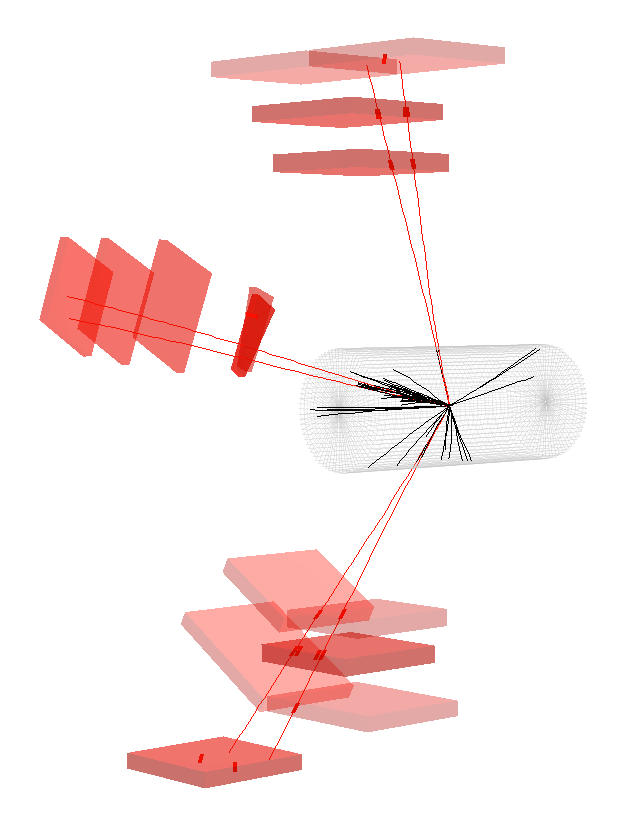
\includegraphics[width=\linewidth]{eventdisplay_3d.png}
\end{columns}

\end{center}
\end{frame}

%% \begin{notes}
%% \item This is the annotated version of my talk.
%% \item If you want the version that I am presenting, download the one
%% labeled ``slides'' on Indico (or just ignore these yellow pages).
%% \item The annotated version is provided for extra detail and a written
%% record of comments that I intend to make orally.
%% \item Yellow notes refer to the content on the {\it previous} page.
%% \item All other slides are identical for the two versions.
%% \end{notes}

\small

\section{Introduction}

\begin{frame}
\frametitle{\only<1>{Generic phenomenology}\only<2>{Dark SUSY example}\only<3>{NMSSM Higgs example}}
\begin{center}
\only<1>{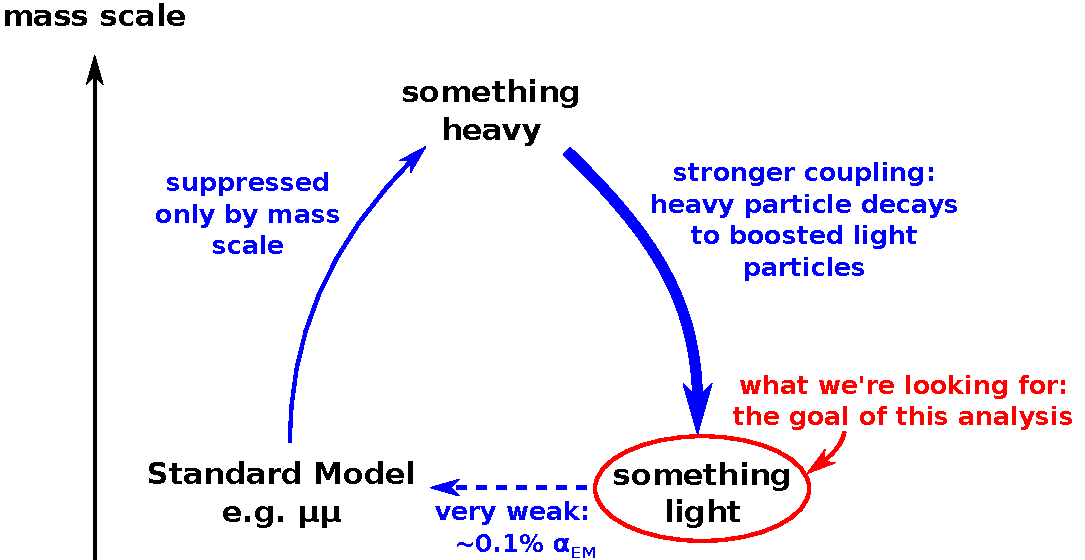
\includegraphics[width=0.9\linewidth]{basic_picture.pdf}}
\only<2>{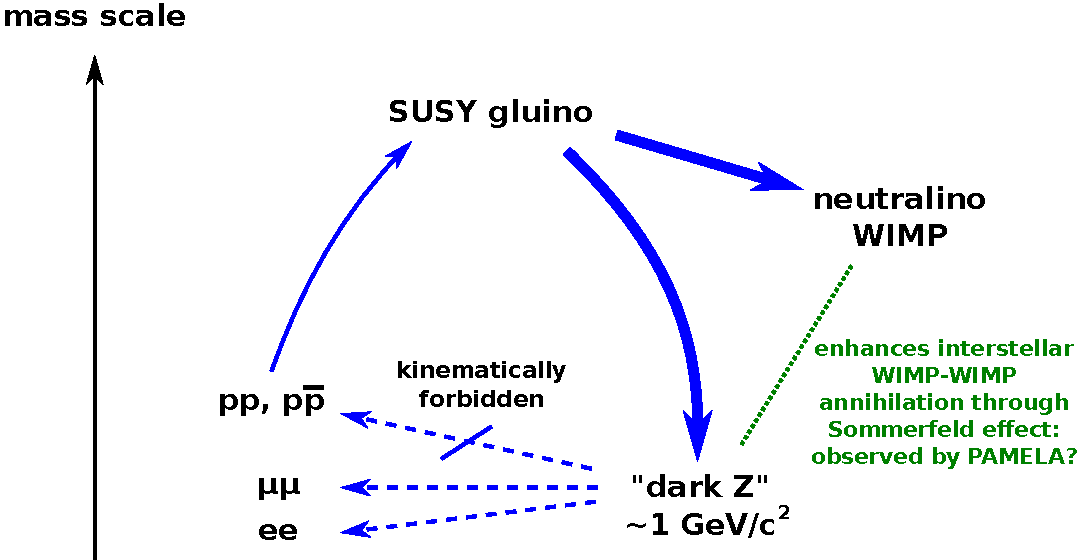
\includegraphics[width=0.9\linewidth]{basic_picture2.pdf}}
\only<3>{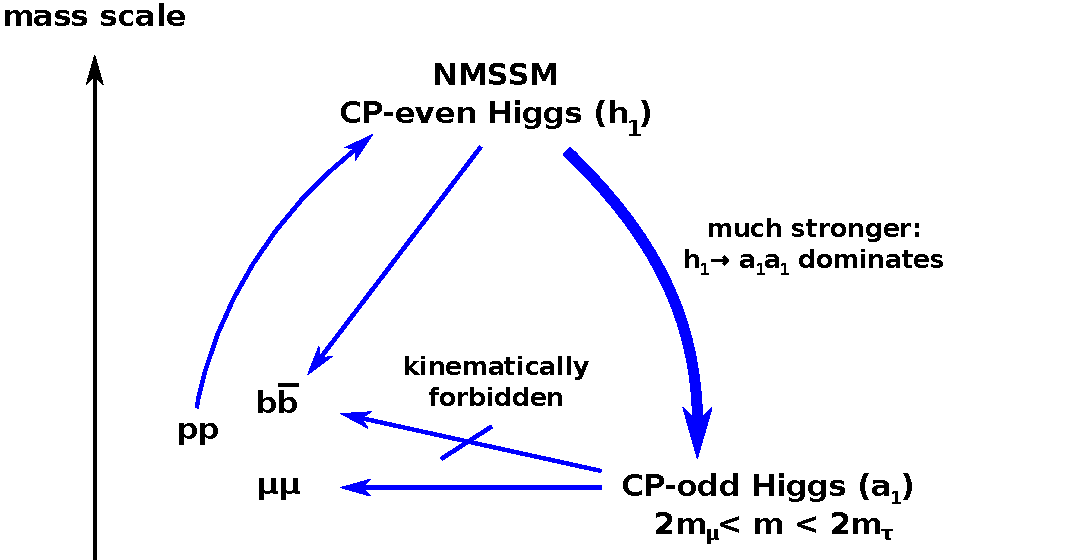
\includegraphics[width=0.9\linewidth]{basic_picture3.pdf}}
\end{center}

\begin{itemize}
\item \only<1>{Generic hidden-valley picture: predicts new low-mass, high-momentum particles decaying to states like $\mu\mu$}\only<2>{Sub-class motivated by PAMELA positron excess (and lack of antiproton excess) when interpreted as WIMP-WIMP annihilation}\only<3>{A region of NMSSM parameter space allows the Higgs to escape LEP limits by decaying to lighter Higgs bosons rather than $b\bar{b}$, $\tau^+\tau^-$, etc.}
\item<3> Same basic picture, same signature
\end{itemize}
\end{frame}

\begin{frame}
\frametitle{Analysis strategy}
\begin{columns}
\column{0.55\linewidth}
Motivated by phenomenology:
\begin{itemize}
\item Hidden sector could have any spectrum, but due to weak coupling,
  only the lightest state decays to Standard Model pairs

\textcolor{darkblue}{$\longrightarrow$ search for a single $m_1$ resonance peak}

\item Visible pairs may overlap, but the light cascades would be
  separated by their boost

\textcolor{darkblue}{$\longrightarrow$ identify well-separated groups, then
  resolve combinatorics}

\item $\mathcal{B}(m_1 \to \mu\mu)$ is likely to be high, but not
  necessarily 100\%

\textcolor{darkblue}{$\longrightarrow$ look for the resonance in
  muons, but don't exclude other particles (e.g.\ with isolation)}
\end{itemize}

\column{0.5\linewidth}
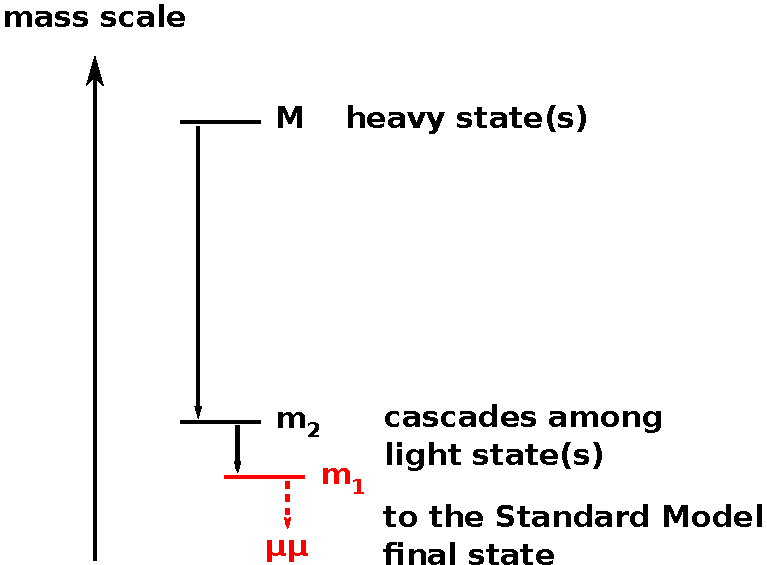
\includegraphics[width=\linewidth]{basic_picture4.pdf}

\begin{center}
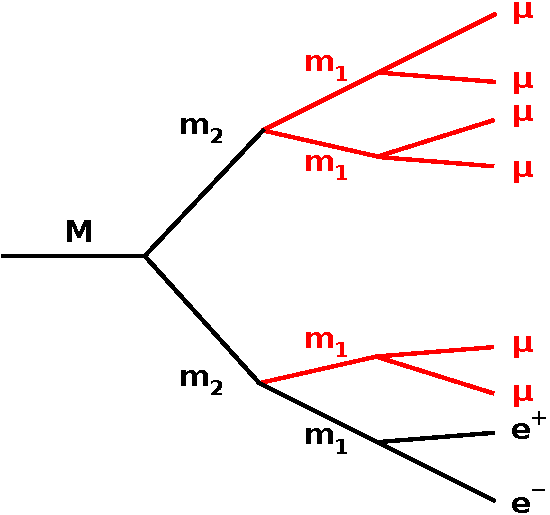
\includegraphics[width=0.7\linewidth]{basic_picture5.pdf}
\end{center}
\end{columns}
\end{frame}

\begin{frame}
\frametitle{Analysis details}
\begin{columns}
\column{0.55\linewidth}
\begin{itemize}
\item Identify groups of muons (``mu-jets'') by mass and momentum
  separately, rather than $\Delta R$, to avoid cutting out large parts
  of phase space

\item Categorize signal topologies by the number and composition of mu-jets: each has different backgrounds

\item Identify the most consistent dimuon mass combinations within
  each mu-jet, look for a resonance peak in all dimuons simultaneously

\item Neither require events to contain hadronic jets, missing energy,
  other leptons, nor exclude them

%% \item Identify groups of at least two muons in a rectangle of mass and
%%   $p_T$ (rather than a $\Delta R$ cut)
%% \item Search for $m_1 \to \mu\mu$ resonance in pairs of these muons (possibly many per event)
%% \item No isolation, as the signal may be $e^+e^-\mu\mu$ as well as $\mu\mu\mu\mu$
%% \item No specific model: search for all event topologies that are
%%   distinct from Standard Model backgrounds
%% \item Inclusive search: 
\end{itemize}

\column{0.37\linewidth}
\vspace{0.1 cm}
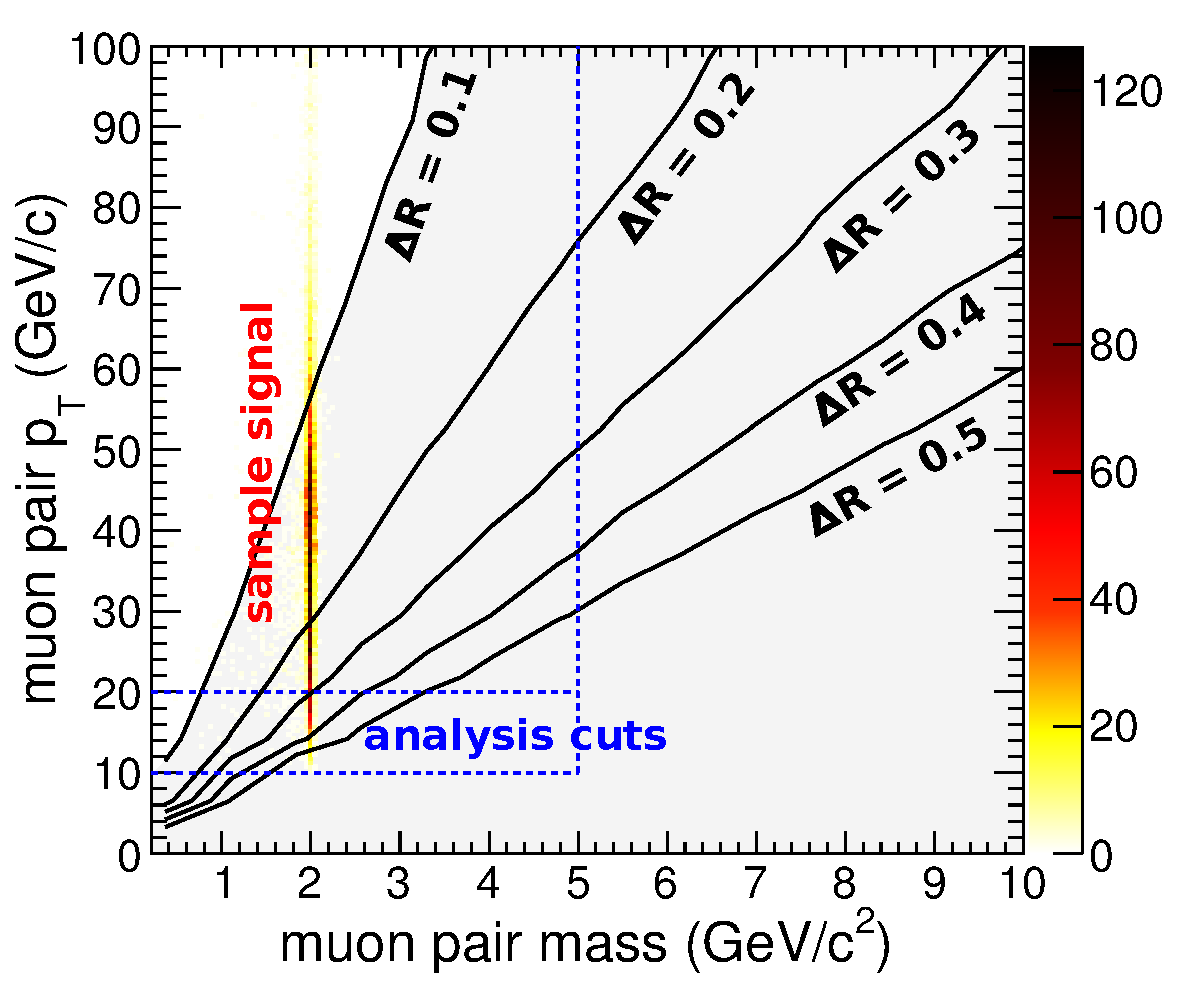
\includegraphics[width=\linewidth]{openingangle_with_signal.pdf}

\vspace{0.3 cm}
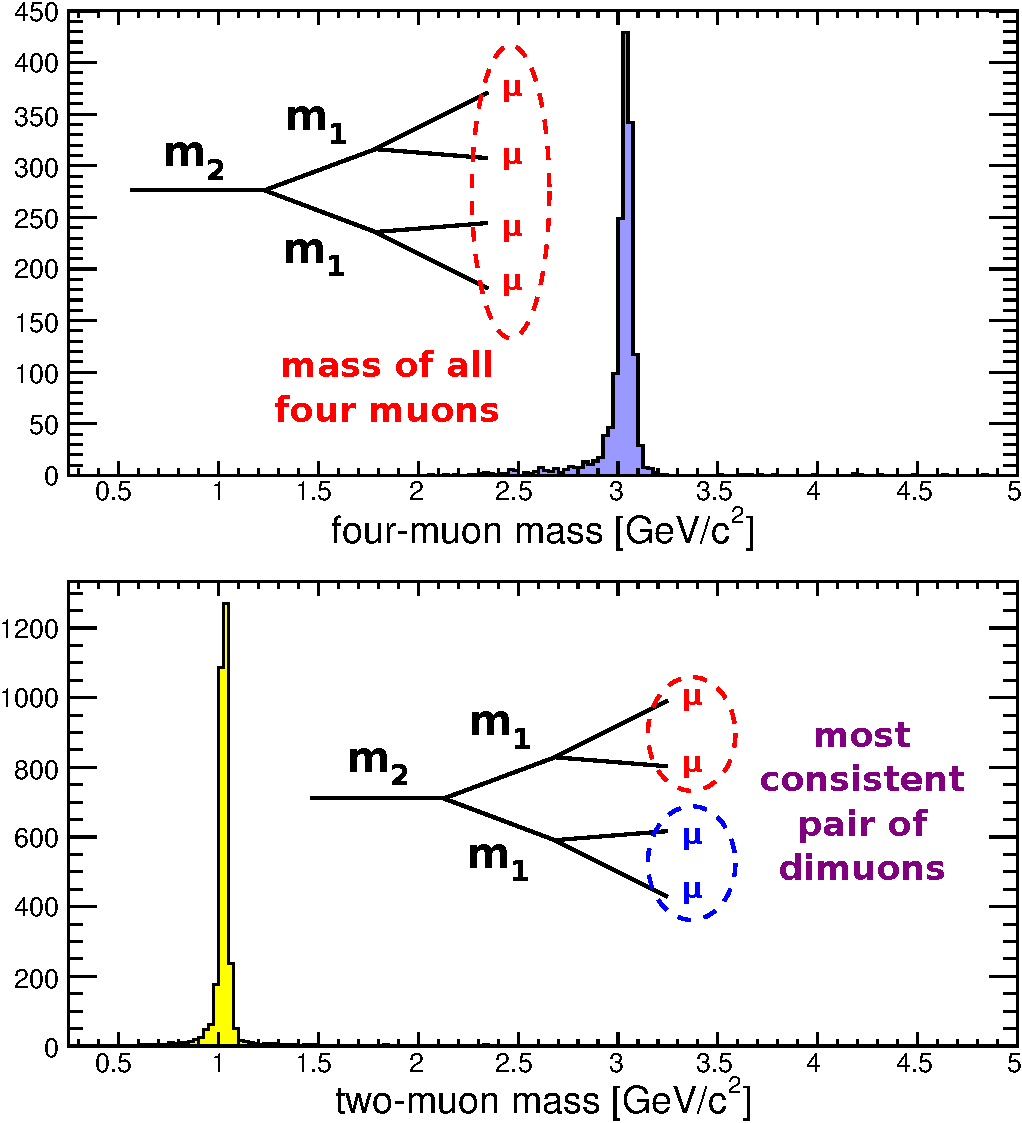
\includegraphics[width=\linewidth]{four-two-muon-mass.pdf}
\end{columns}
\end{frame}

\begin{frame}
\frametitle{Signal topologies}

\vspace{1 cm}
\hfill 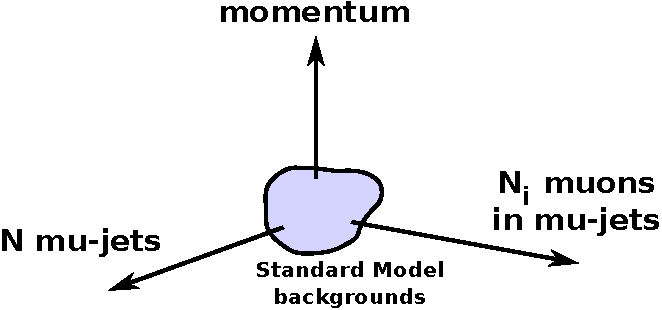
\includegraphics[width=0.5\linewidth]{signal_regions.pdf}

\vspace{-3.5 cm}
\begin{itemize}
\item Look for a new resonance in all channels with small backgrounds

\item Any one of the following reduce \\ Standard Model backgrounds to $\mathcal{O}(1\mbox{ pb})$:
\begin{itemize}
\item $p_T \gtrsim 100$~GeV/$c$
\item $\ge 2$ mu-jets in an event
\item $\ge 4$ muons in a mu-jet
\end{itemize}
\item Define non-overlapping signal regions:
\end{itemize}

\vspace{-0.5 cm}
\begin{center}
\begin{minipage}{0.8\linewidth}
\scriptsize
\begin{enumerate}[(\alph{enumi})]
\item exactly one mu-jet per event
\begin{enumerate}[(\scriptsize \mbox{a}-\arabic{enumii})]
\item \scriptsize $p_T > 80$~GeV/$c$ mu-jet containing two muons \mbox{($m_1 \to 2\mu$)\hspace{-1 cm}}
\item \scriptsize any mu-jet containing four muons ($m_2 \to m_1 m_1 \to 4\mu$)
\item \scriptsize more than four
\end{enumerate}

\item two mu-jets per event
\begin{enumerate}[\scriptsize (b-\arabic{enumii})]
\item \scriptsize $2\mu$, $2\mu$ ($M \to m_1 m_1$, which is the NMSSM signature)
\item \scriptsize $2\mu$, $4\mu$ ($M \to m_1 m_2$)
\item \scriptsize $4\mu$, $4\mu$ ($M \to m_2 m_2$)
\item \scriptsize either has more than four
\end{enumerate}

\item \scriptsize more than two mu-jets per event
\end{enumerate}
\end{minipage}
\end{center}
\end{frame}

\begin{frame}
\frametitle{Signal extraction}

\begin{itemize}
\item Use the fact that a real $m_1$ mass must be equal for all
  dimuons, while the background is uncorrelated
\begin{itemize}
\item topologies with $n$ dimuons per event form an $n$-dimensional
  space of observables
\item signal is a sharp peak somewhere along the diagonal
\item background distribution is a Cartesian product of shapes derived from data
\end{itemize}

\begin{center}
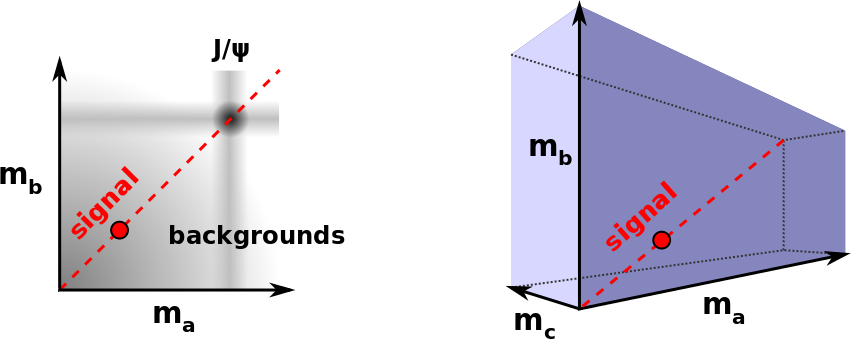
\includegraphics[width=0.9\linewidth]{diagonal.png}
\end{center}

\item Fit to both components yields a data-driven background estimate
  and a signal limit/discovery with the same data
\end{itemize}
\end{frame}

\begin{frame}
\frametitle{Outline for the rest of the talk}
\begin{itemize}\setlength{\itemsep}{0.75 cm}
\item Detector issues; choosing an appropriate acceptance region
\item Understanding the low-mass dimuon mass spectrum
\item Deriving background shape templates
\item Fit results in control regions
\end{itemize}
%% \hspace{-0.83 cm} \textcolor{darkblue}{\Large Outline2}
\end{frame}

\section*{Detector issues}
\begin{frame}

\vfill
\begin{center}
\Huge \textcolor{blue}{Detector issues}
\end{center}

\vfill
Summary of Oct 4 $\mu$POG talk:

\textcolor{blue}{\url{http://indico.cern.ch/conferenceDisplay.py?confId=94649}}
\end{frame}

\begin{frame}
\frametitle{Reconstruction efficiency}

\begin{itemize}
\item We don't use GlobalMuons because they are inefficient for good
  muons {\scriptsize ($p_T > 5$~GeV/$c$, $|\eta| < 2.4$)} that cross
  in the muon system
\begin{itemize}
\item plot efficiency vs.\ distance between muons in the muon system:
\end{itemize}
\end{itemize}

\begin{columns}
\column{0.5\linewidth}
\centering GlobalMuons

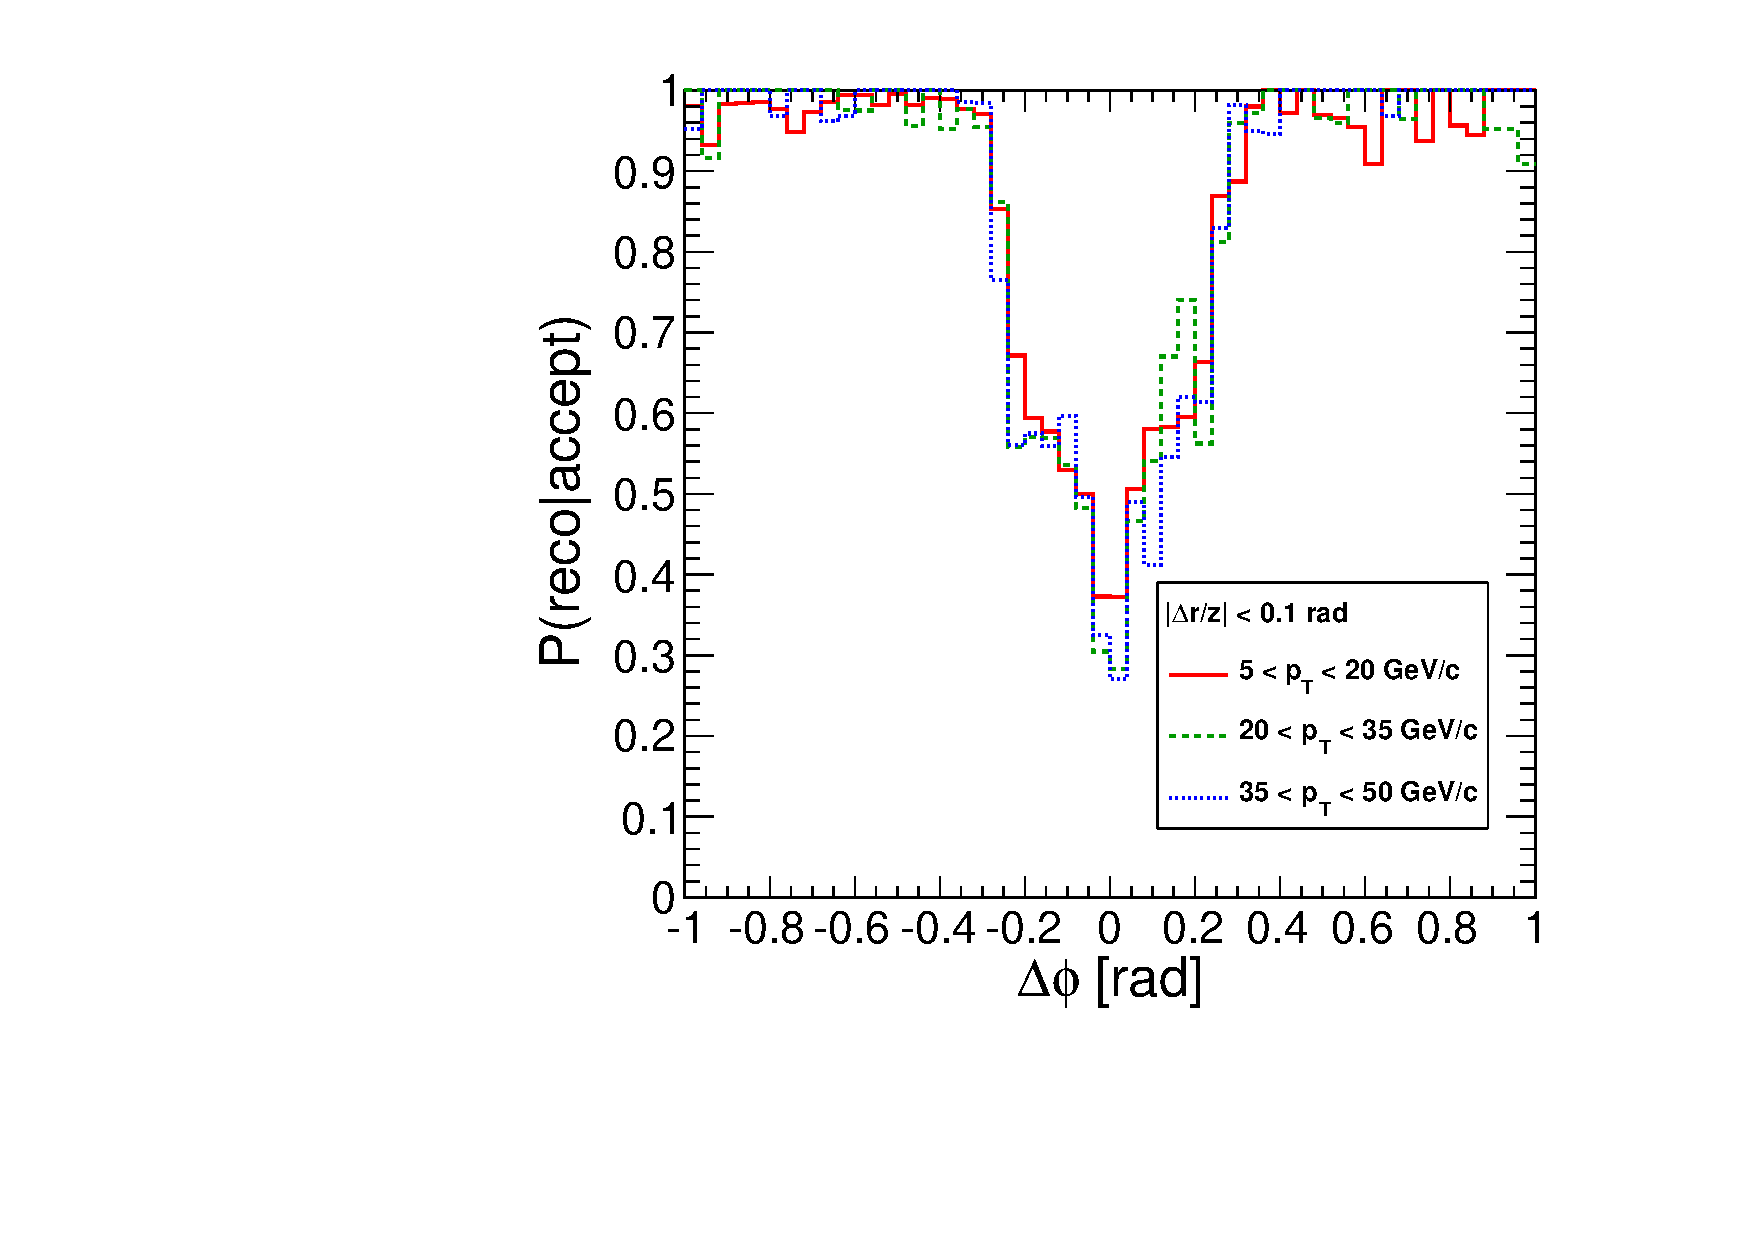
\includegraphics[width=\linewidth]{efficiency_globalmuons.pdf}

\column{0.5\linewidth}
\centering quality TrackerMuons

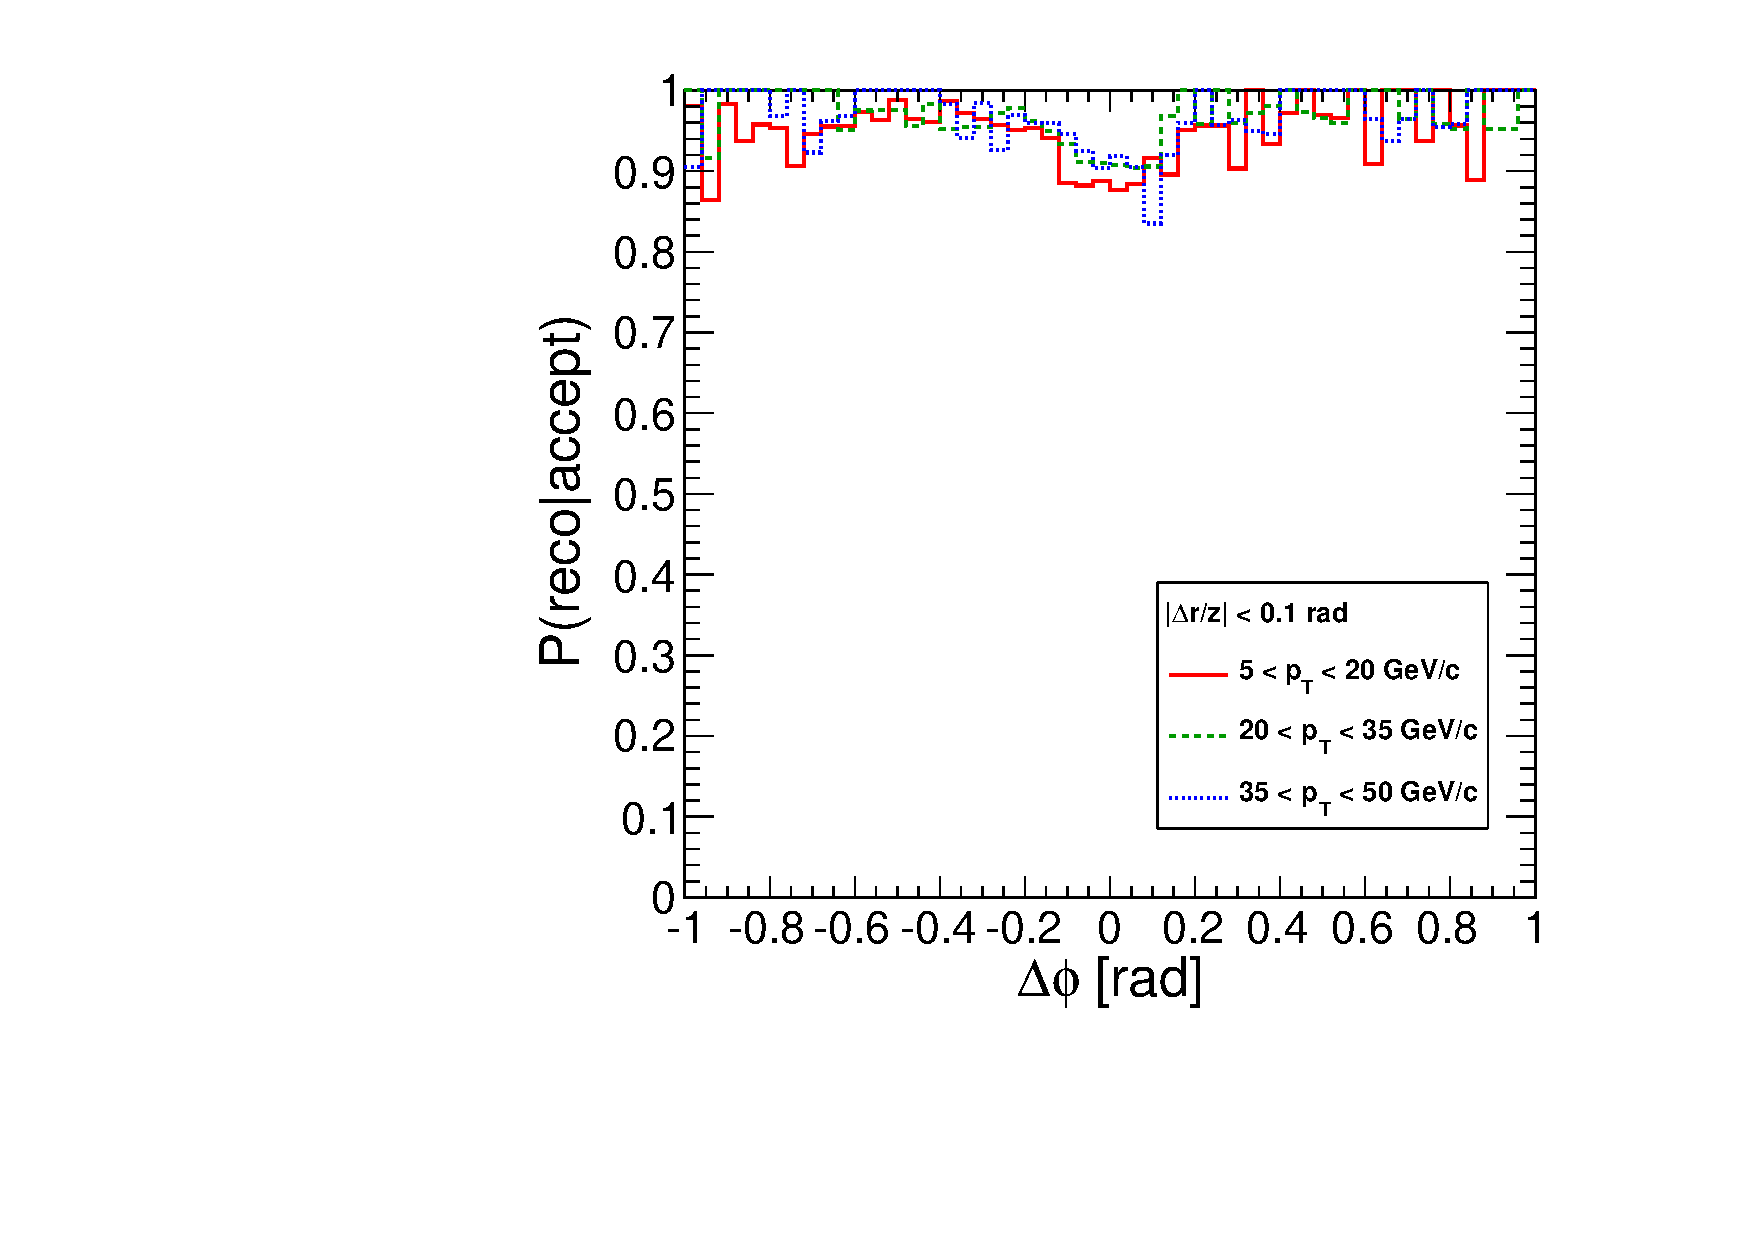
\includegraphics[width=\linewidth]{efficiency_trackermuons.pdf}
\end{columns}

\begin{itemize}
\item We instead use ``quality TrackerMuons'' {\scriptsize ($\ge$ 2
  arbitrated segments, \\ $\ge$ 8 tracker hits, $\chi^2/N_\s{dof} < 4$)},
  which have the same low fake-rate as GlobalMuons, yet high
  efficiency for close-by muons
\end{itemize}
\end{frame}

\begin{frame}
\frametitle{Trigger efficiency}

\begin{itemize}
\item Lowest unprescaled, unisolated, single-muon trigger: HLT\_Mu15
\item Single-muon trigger efficiency is highly dependent on whether the
  muon trajectories cross in the CSCs (endcap only)
\end{itemize}

\begin{columns}
\column{0.45\linewidth}
\centering muons cross each other

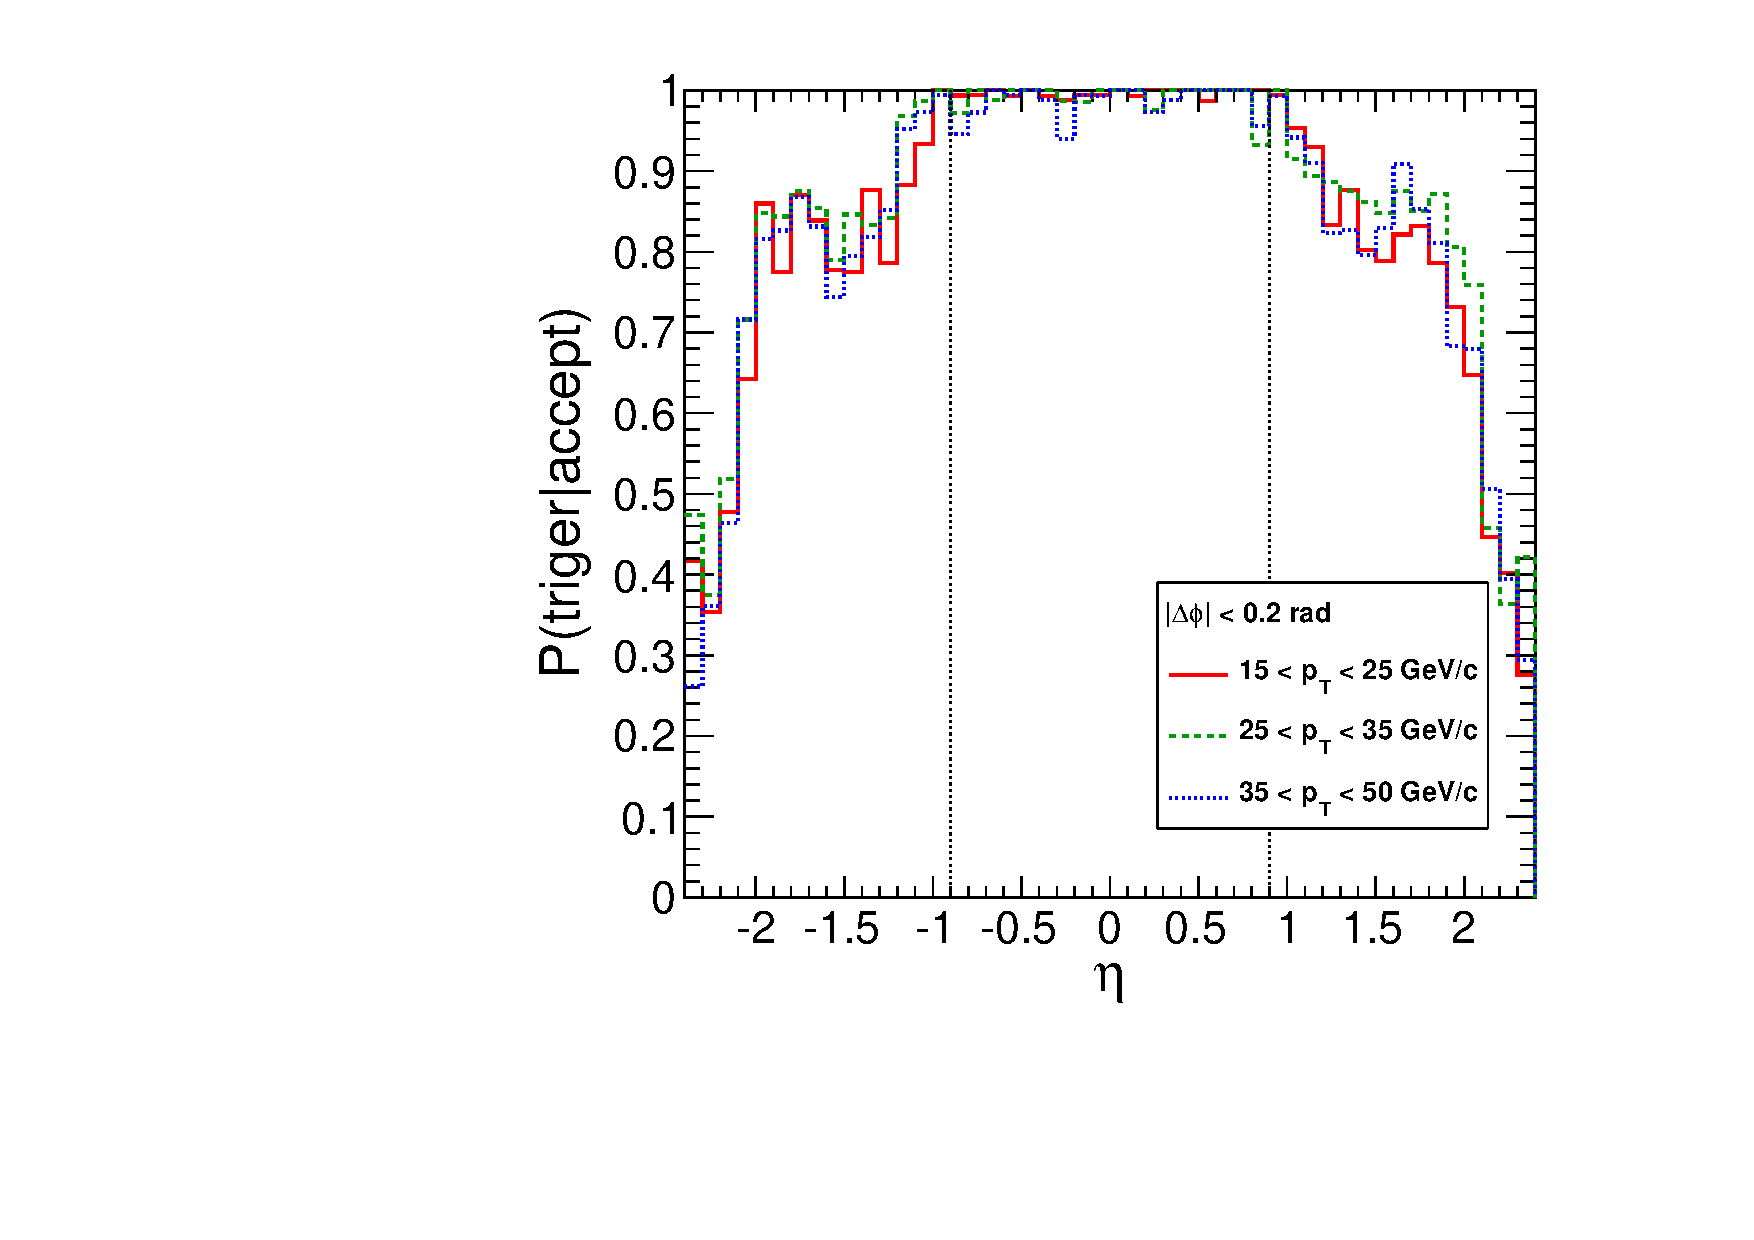
\includegraphics[width=\linewidth]{efficiency_trigger.pdf}

\column{0.45\linewidth}
\centering muons do not cross

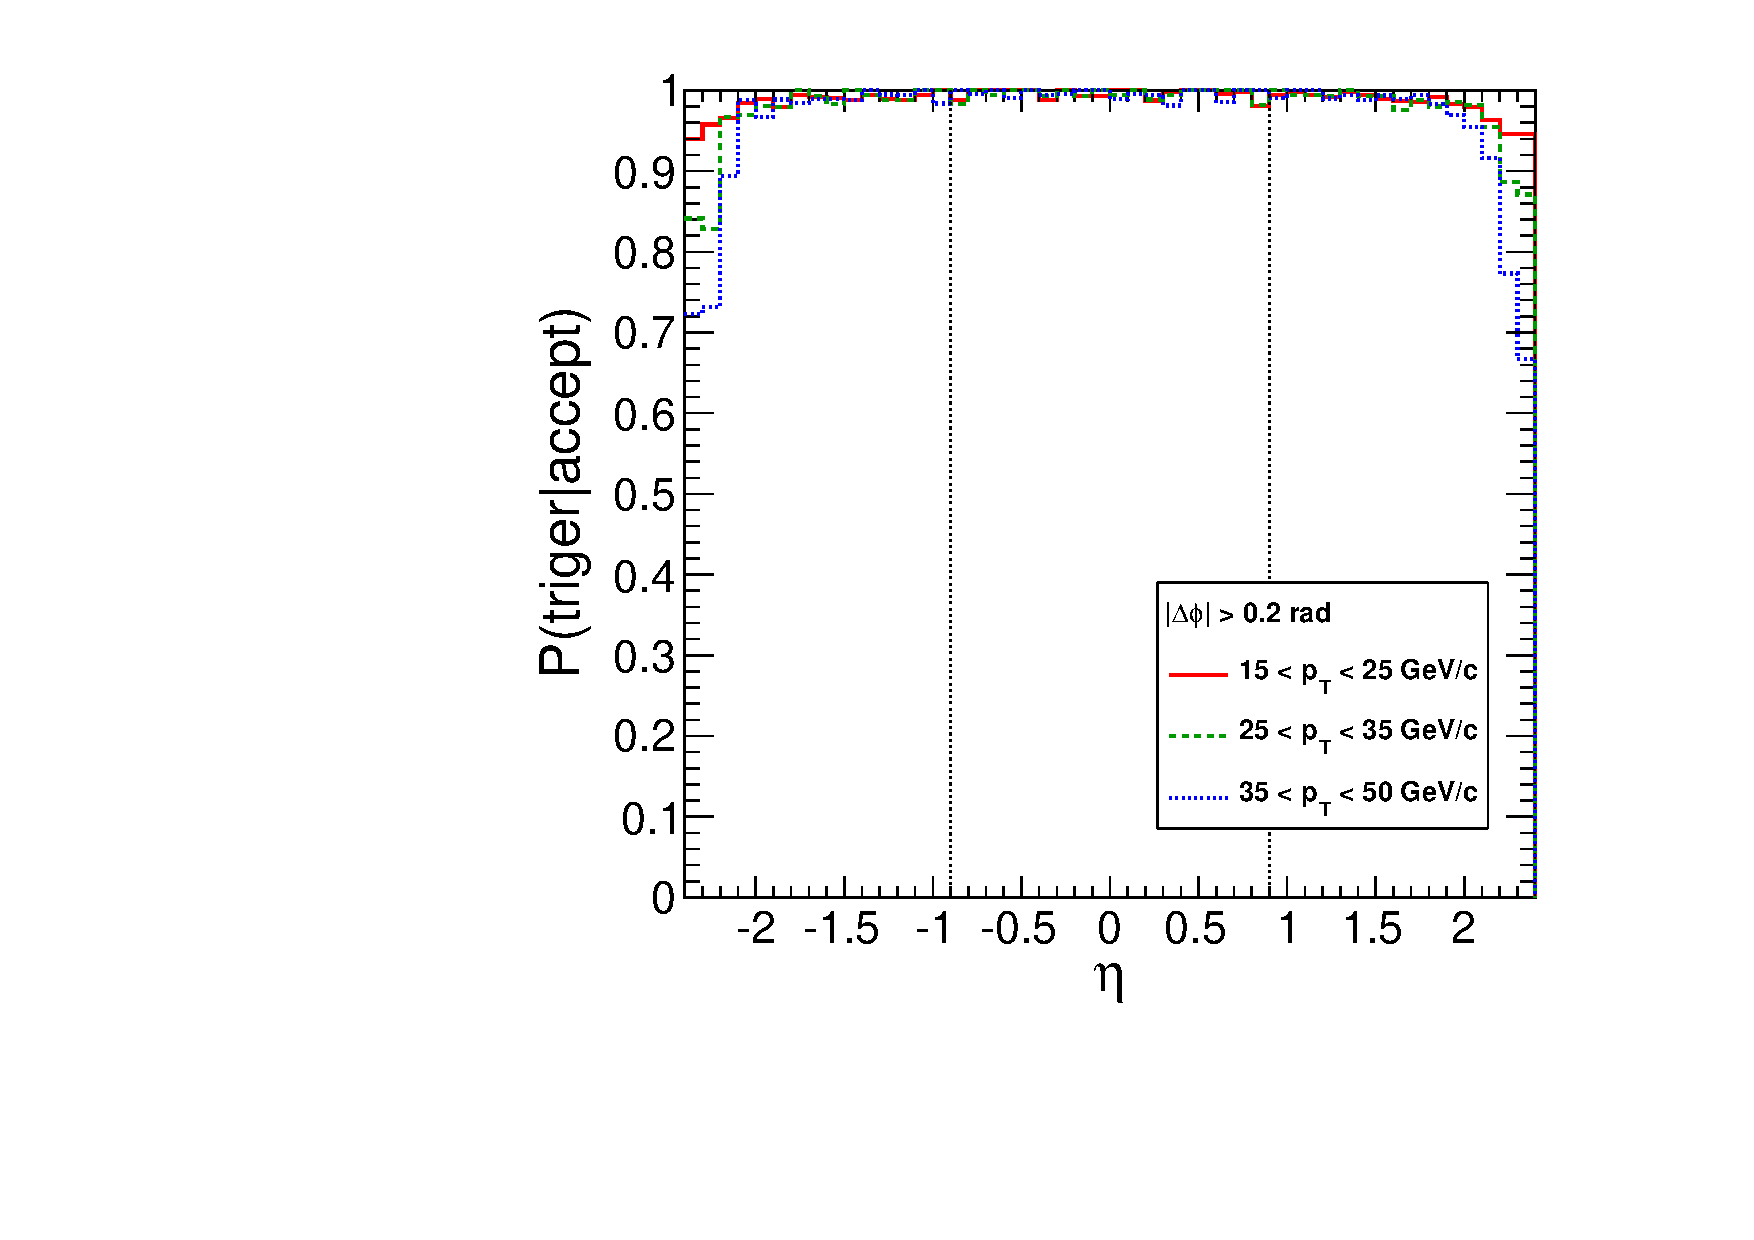
\includegraphics[width=\linewidth]{efficiency_trigger_anticut.pdf}
\end{columns}

\begin{itemize}
\item Trajectory-crossing depends on the precise kinematics of the
  events, which depends on the theoretical model in question
\item Most models predict higher momentum, lower mass than $J/\psi$:
  tag-and-probe would underestimate the inefficiency for those models
\end{itemize}
\end{frame}

\begin{frame}
\frametitle{Acceptance definition}

\begin{itemize}
\item We therefore require at least one $p_T > 15$~GeV/$c$, $|\eta| <
  0.9$ (barrel) muon offline
\begin{itemize}
\item post-acceptance trigger efficiency is $\sim$97\% and independent
  of model kinematics
\item all other muons are much looser: $p_T > 5$~GeV$/c$, $|\eta| < 2.4$
\end{itemize}

\item Provides for a robust analysis at the expense of acceptance

\hfill \mbox{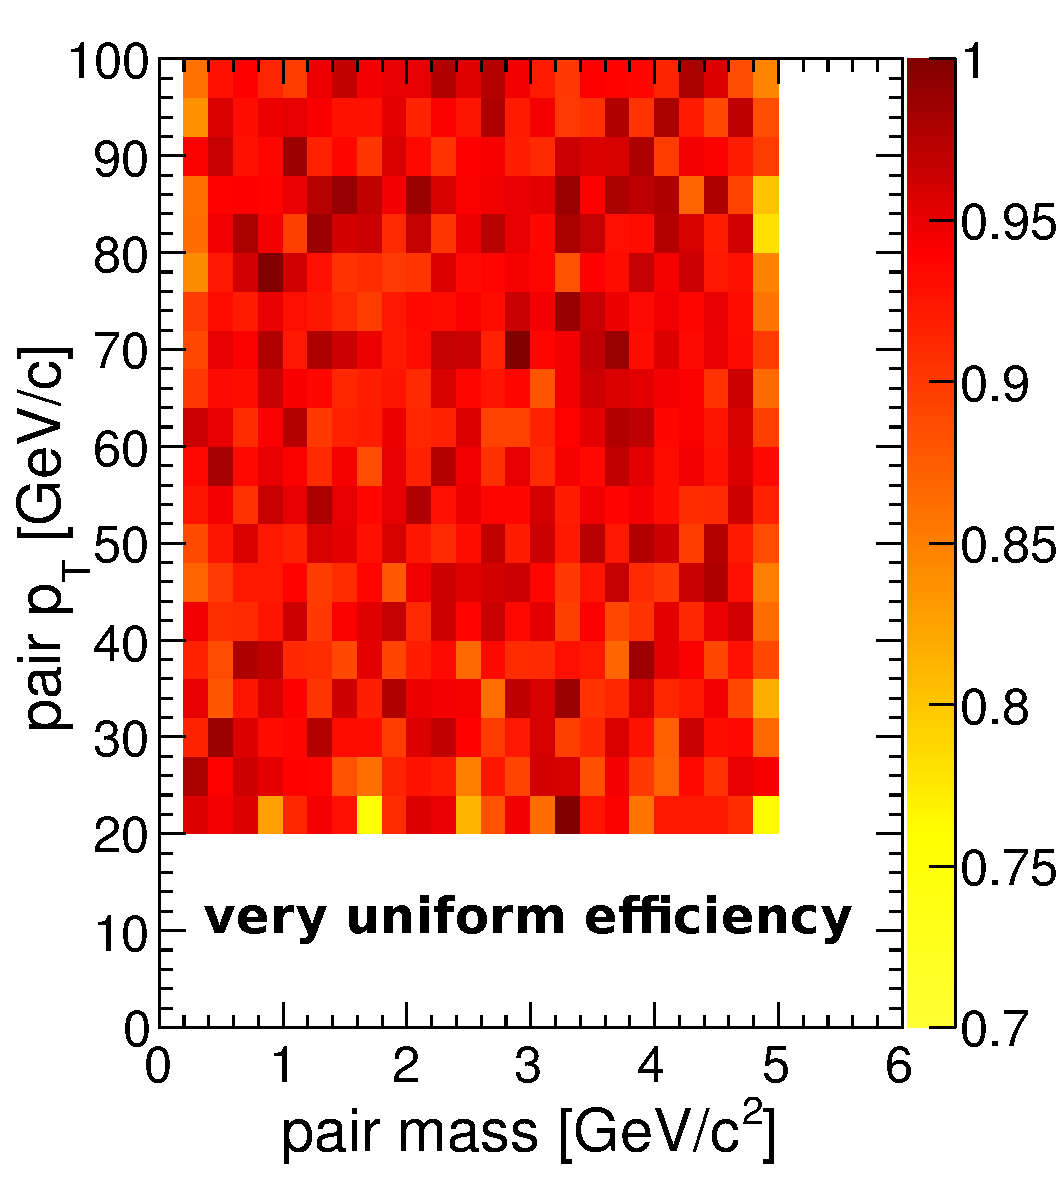
\includegraphics[width=0.37\linewidth]{eff_mujetreco_inplateau_masspt.pdf}\hspace{-0.5 cm}}

\vspace{-4.3 cm}
\item Each signal region specifies additional cuts \\ on the number and
  properties of mu-jets

\item Mu-jets are built recursively from \\ opposite sign muon pairs with
\begin{itemize}
\item pairwise invariant mass $<$ 5~GeV/$c^2$
\item vertex $\chi^2$ probability $>$ 1\%
\item $\Delta R < 0.01$ (tiny) if the above fail
\end{itemize}

\item $\sim$99\% mu-jet forming efficiency, \\ $\sim$95\% folding in
  reconstruction of two muons (right)
\end{itemize}
\end{frame}

\section*{Understanding the low-mass dimuon spectrum}
\begin{frame}
\vspace{0.75 cm}
\begin{center}
\Huge \textcolor{blue}{Understanding the low-mass dimuon spectrum}

\vspace{0.25 cm}
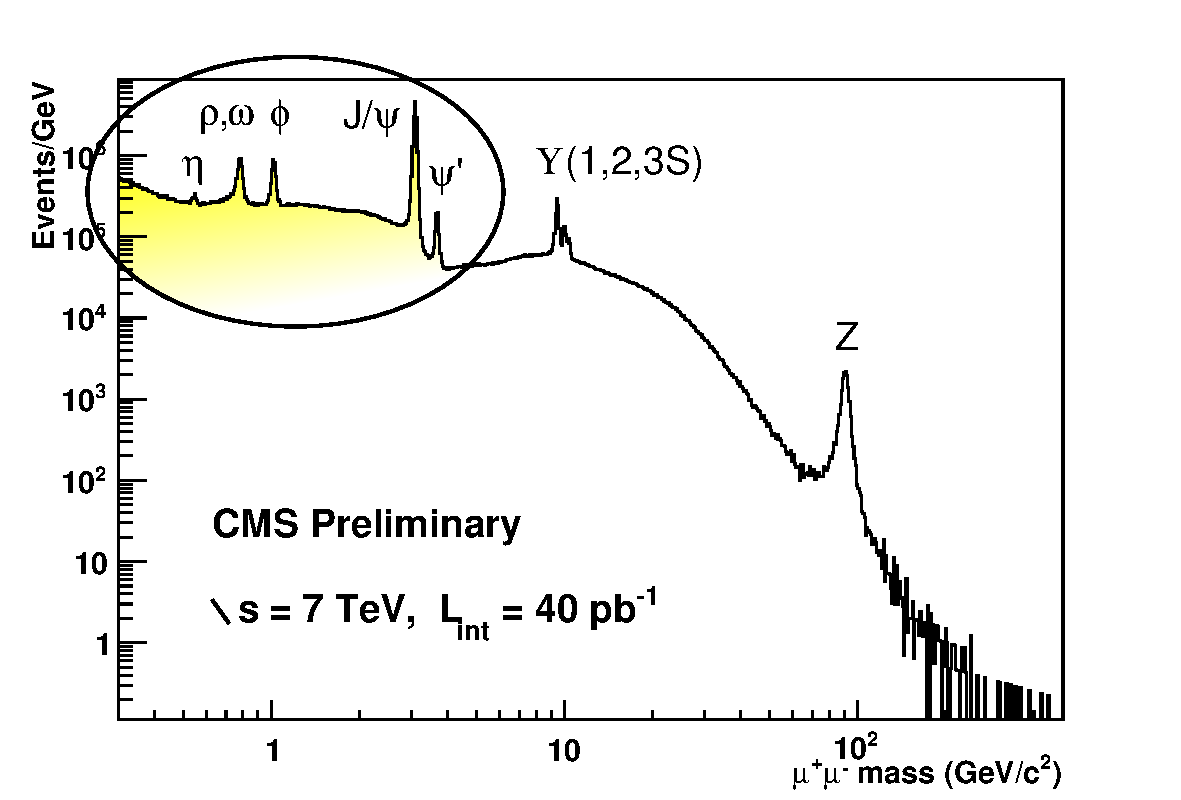
\includegraphics[width=0.75\linewidth]{dimuonSpectrum_40pb-1.pdf}
\end{center}
\end{frame}

\begin{frame}
\frametitle{Low-mass dimuons}

\vspace{0.25 cm}
\hfill 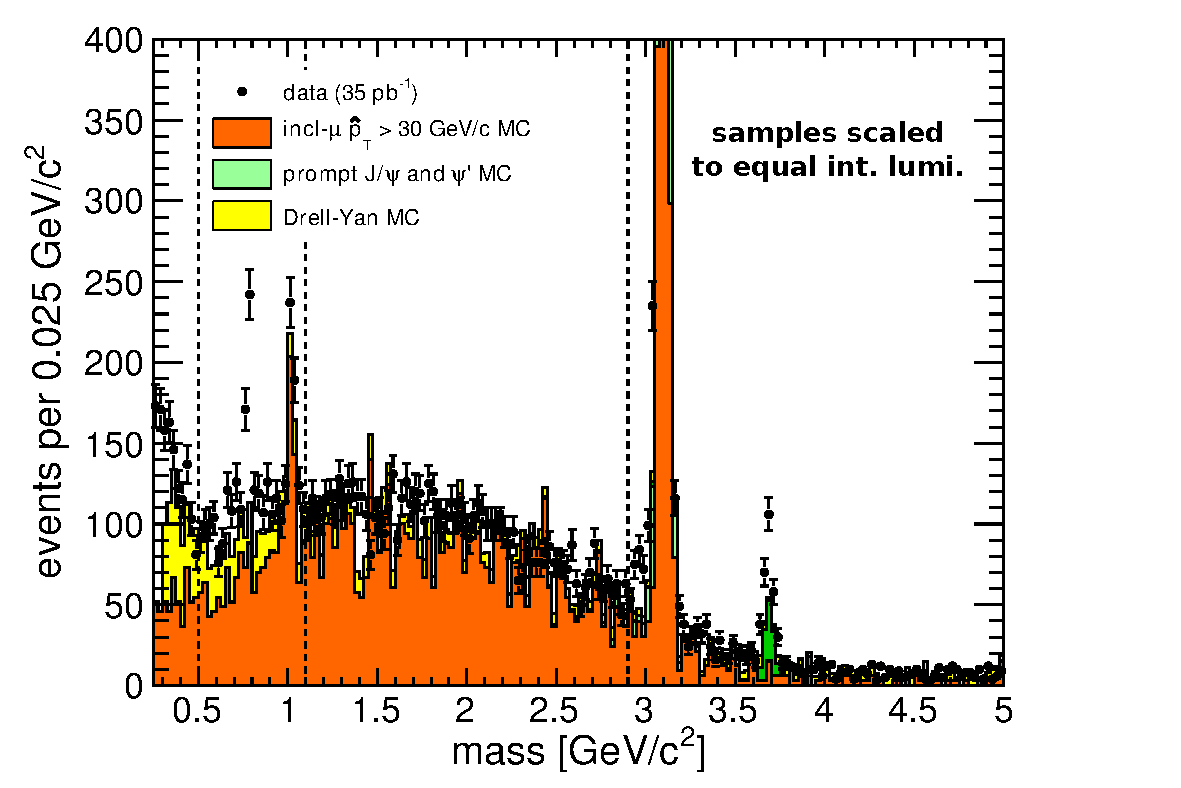
\includegraphics[width=0.5\linewidth]{support_mass_all.pdf}

\vspace{-3.7 cm}
\begin{itemize}
\item ``Raw'' mass spectrum has \\ several components:
\begin{itemize}
\item resonances (prompt and \\ from $b$ decays)
\item double-semileptonic \\ $b \to \mu\mu X$ continuum
\item low-mass Drell-Yan
\end{itemize}

\item MC isn't perfect: study data/MC differences using isolation (defined
  such that $\mu\mu$ doesn't self-veto) and distance of flight ($L_{xy}$)
\end{itemize}

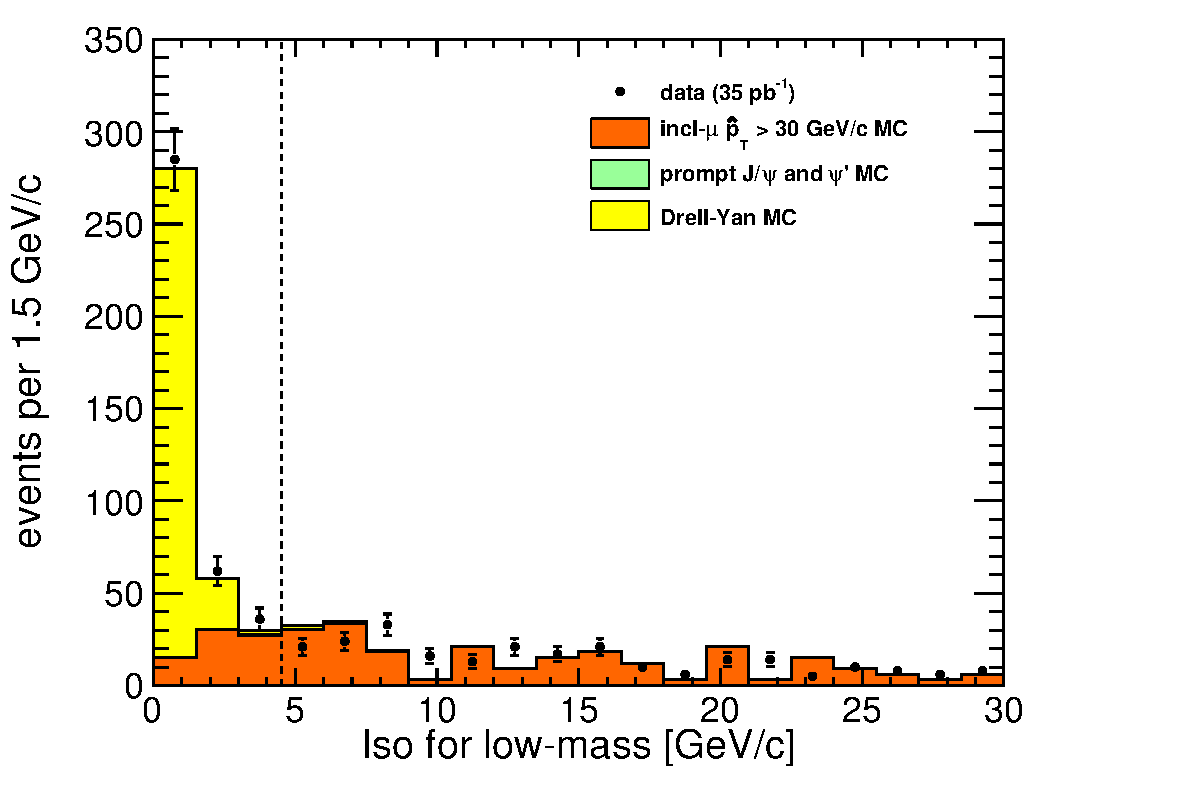
\includegraphics[width=0.5\linewidth]{support_iso_lowmass.pdf}
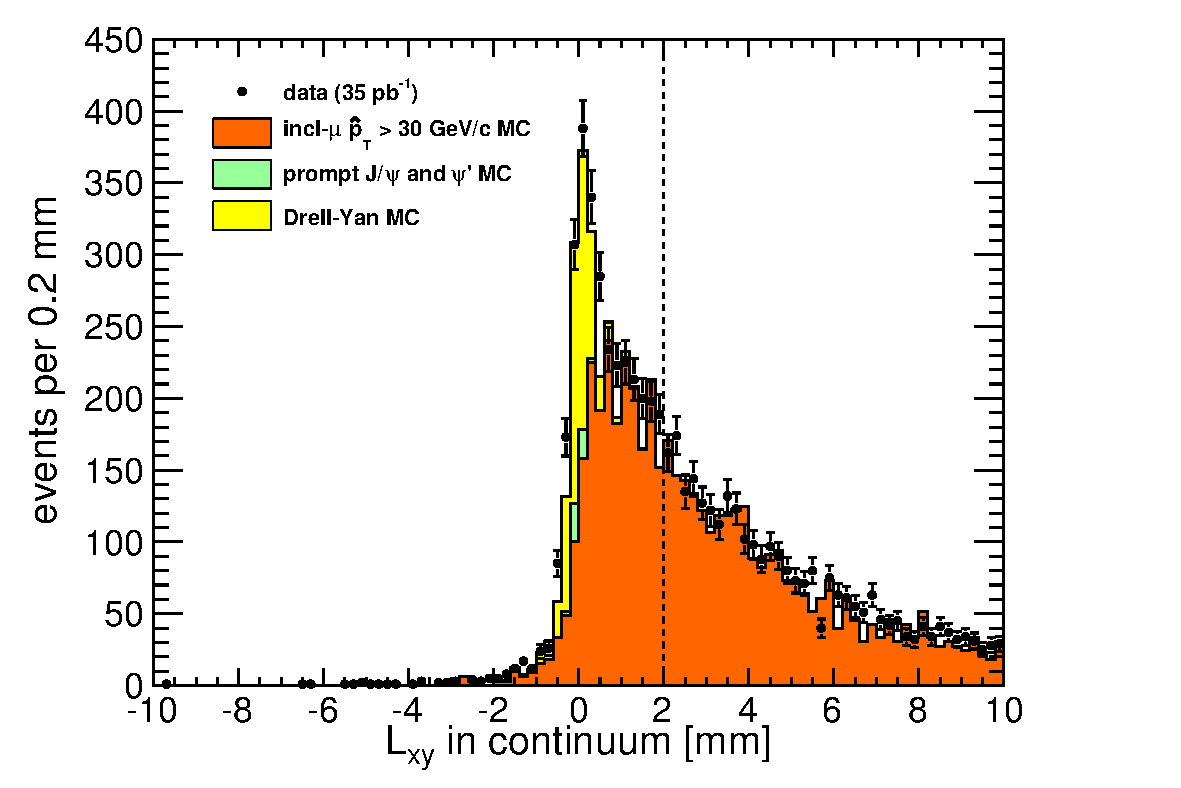
\includegraphics[width=0.5\linewidth]{support_lxy_continuum.pdf}
\end{frame}

\begin{frame}
\frametitle{Low-mass dimuons}

\begin{itemize}
\item Split sample into $b\bar{b}$ and Drell-Yan/prompt resonances with this cut:

\mbox{ } \hfill $Iso > 4.5$~GeV/$c$ {\bf or} $L_{xy} > 2$~mm \hfill \mbox{ }
\label{pag:bbcuts}
\end{itemize}

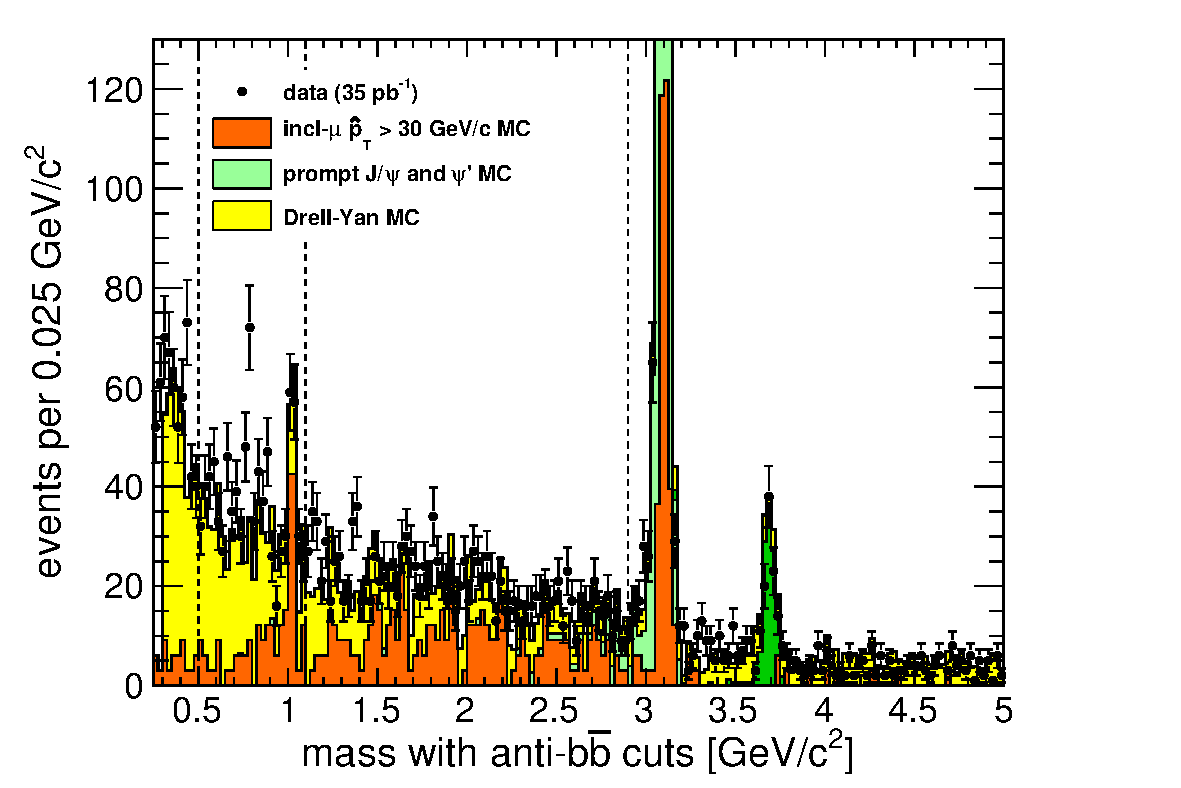
\includegraphics[width=0.5\linewidth]{support_mass_antibbbar.pdf}
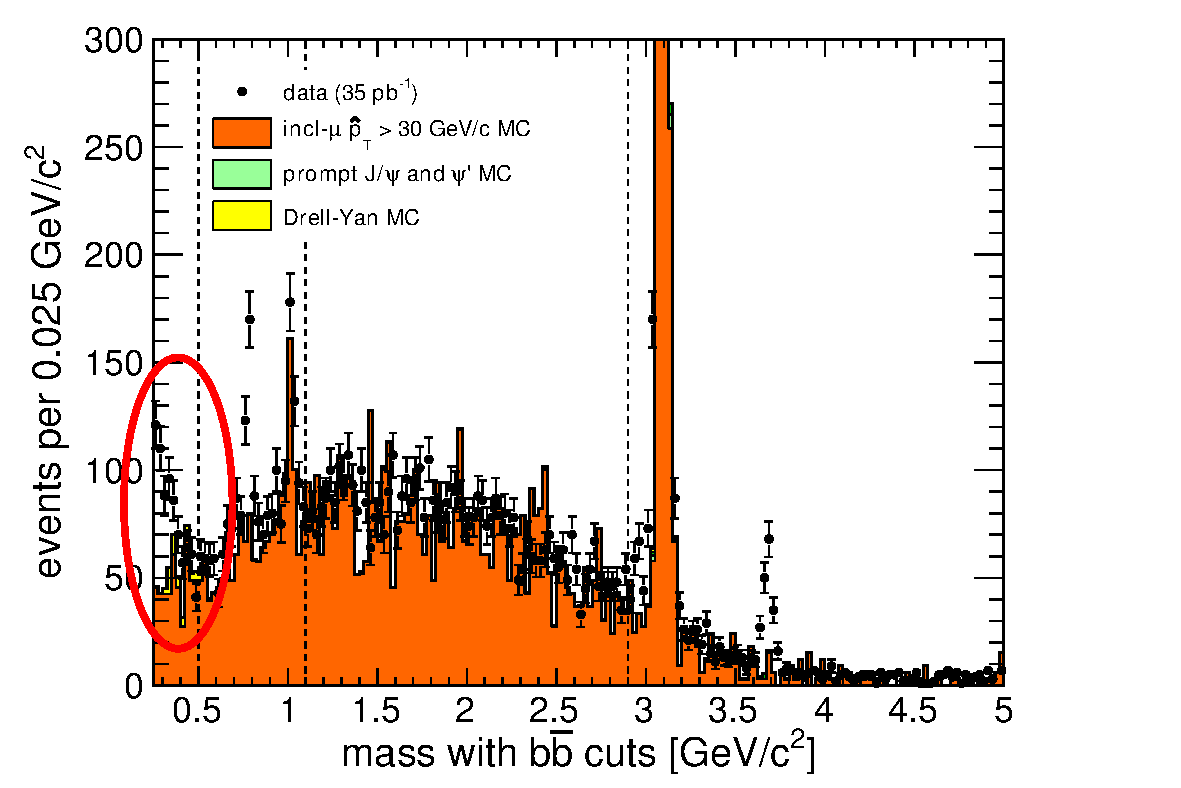
\includegraphics[width=0.5\linewidth]{support_mass_bbbar.pdf}

\begin{itemize}
\item Much of the low-mass spectrum is Drell-Yan (not in any official samples, so we generated it with Pythia 8)
\item Some resonances are not in inclusive-muon MC: $\omega(782)$, $\psi'(3686)$
\item There's also a low-mass excess \textcolor{red}{(red circle)} not shaped like a resonance peak
\end{itemize}
\end{frame}

\begin{frame}
\frametitle{The low-mass excess}

\begin{itemize}
\item The excess is a broad spectrum with an endpoint below $m_\eta = 0.55$~GeV/$c^2$: could be $\eta \to \mu\mu\gamma$
\item $\mathcal{B}(\eta \to \mu\mu\gamma) = 3\times 10^{-4} \approx \mathcal{B}(\omega \to \mu\mu) \approx \mathcal{B}(\phi \to \mu\mu)$
\item Search for exactly one PF-photon in $\Delta R < 0.1$, plot $\mu\mu\gamma$ spectrum
\end{itemize}

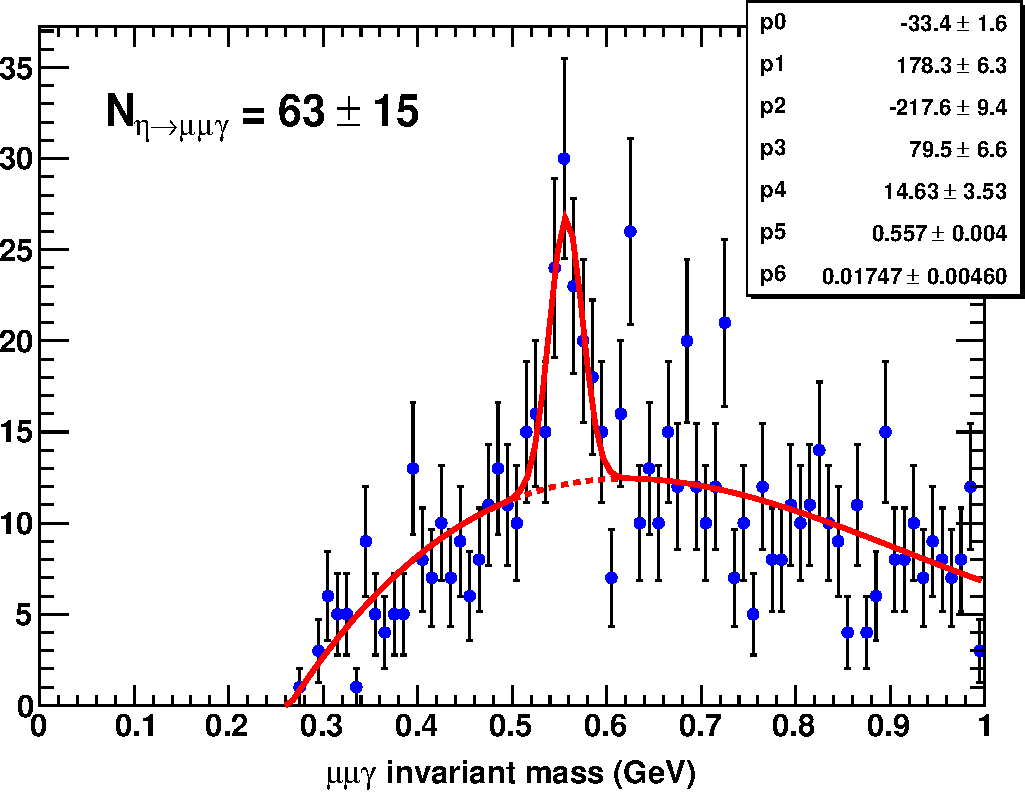
\includegraphics[height=4.7 cm]{eta_peak.pdf} \hfill
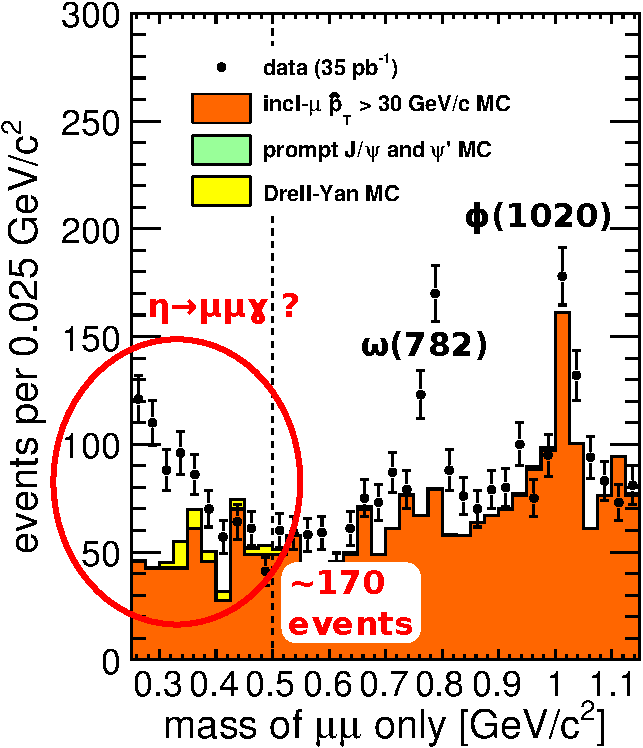
\includegraphics[height=4.7 cm]{mass_of_mumu_only.pdf}

\begin{itemize}
\item $\eta \to \mu\mu\gamma$ accounts for at least 1/3 of the excess
\item We will assume that it is a part of the background
\end{itemize}
\end{frame}

\section*{Background shape templates}
\begin{frame}
\begin{center}
\Huge \textcolor{blue}{Background shape templates}
\end{center}
\end{frame}

\begin{frame}
\frametitle{Method}

\begin{itemize}
\item Signal + background fits determine the number of background
  events in the signal regions, but with too few events to also
  determine the shapes
\end{itemize}

\vspace{-0.45 cm}
\hfill 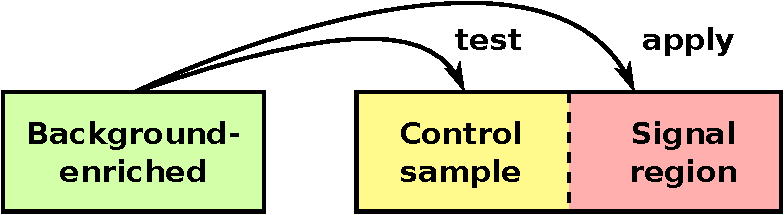
\includegraphics[width=0.5\linewidth]{bkgnd_control_signal.pdf}

\vspace{-1.6 cm}
\begin{enumerate}
\item Get the shapes from \\ ``background-enriched'' \\ samples with the same \\ kinematics, constructed \\ from large-statistics samples that have the same physics content

\item Test template shapes in control samples close to the signal regions

\item Use background $B(m_a, m_b)$ and signal $S(m_a, m_b; m_1)$ shapes in the signal region fits:

\mbox{ } \hfill $\alpha B(m_a, m_b) + \beta S(m_a, m_b; m_1)$ \hfill \mbox{ }
\end{enumerate}

\begin{itemize}
\item Background estimate is effectively a sideband with a known shape
\end{itemize}
\end{frame}

\begin{frame}
\frametitle{Region (a-1): high-$p_T$ dimuon}

\hfill 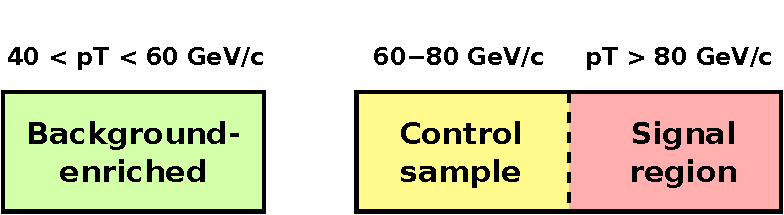
\includegraphics[width=0.5\linewidth]{bkgnd_control_signal_a-1.pdf}

\vspace{-1.5 cm}
\begin{itemize}
\item For the single, high-$p_T$ \\ dimuon case, get the \\ background shape from \\ lower-$p_T$ dimuon spectrum
\item Above 40~GeV/$c$, $b\bar{b}$ to non-$b\bar{b}$ ratio is constant (see backup)
\item Fit background-enriched sample to a smooth curve, overlay the fitted curve on control sample, allowing only normalization to float:
\end{itemize}

\begin{columns}
\column{0.5\linewidth}
\centering background-enriched

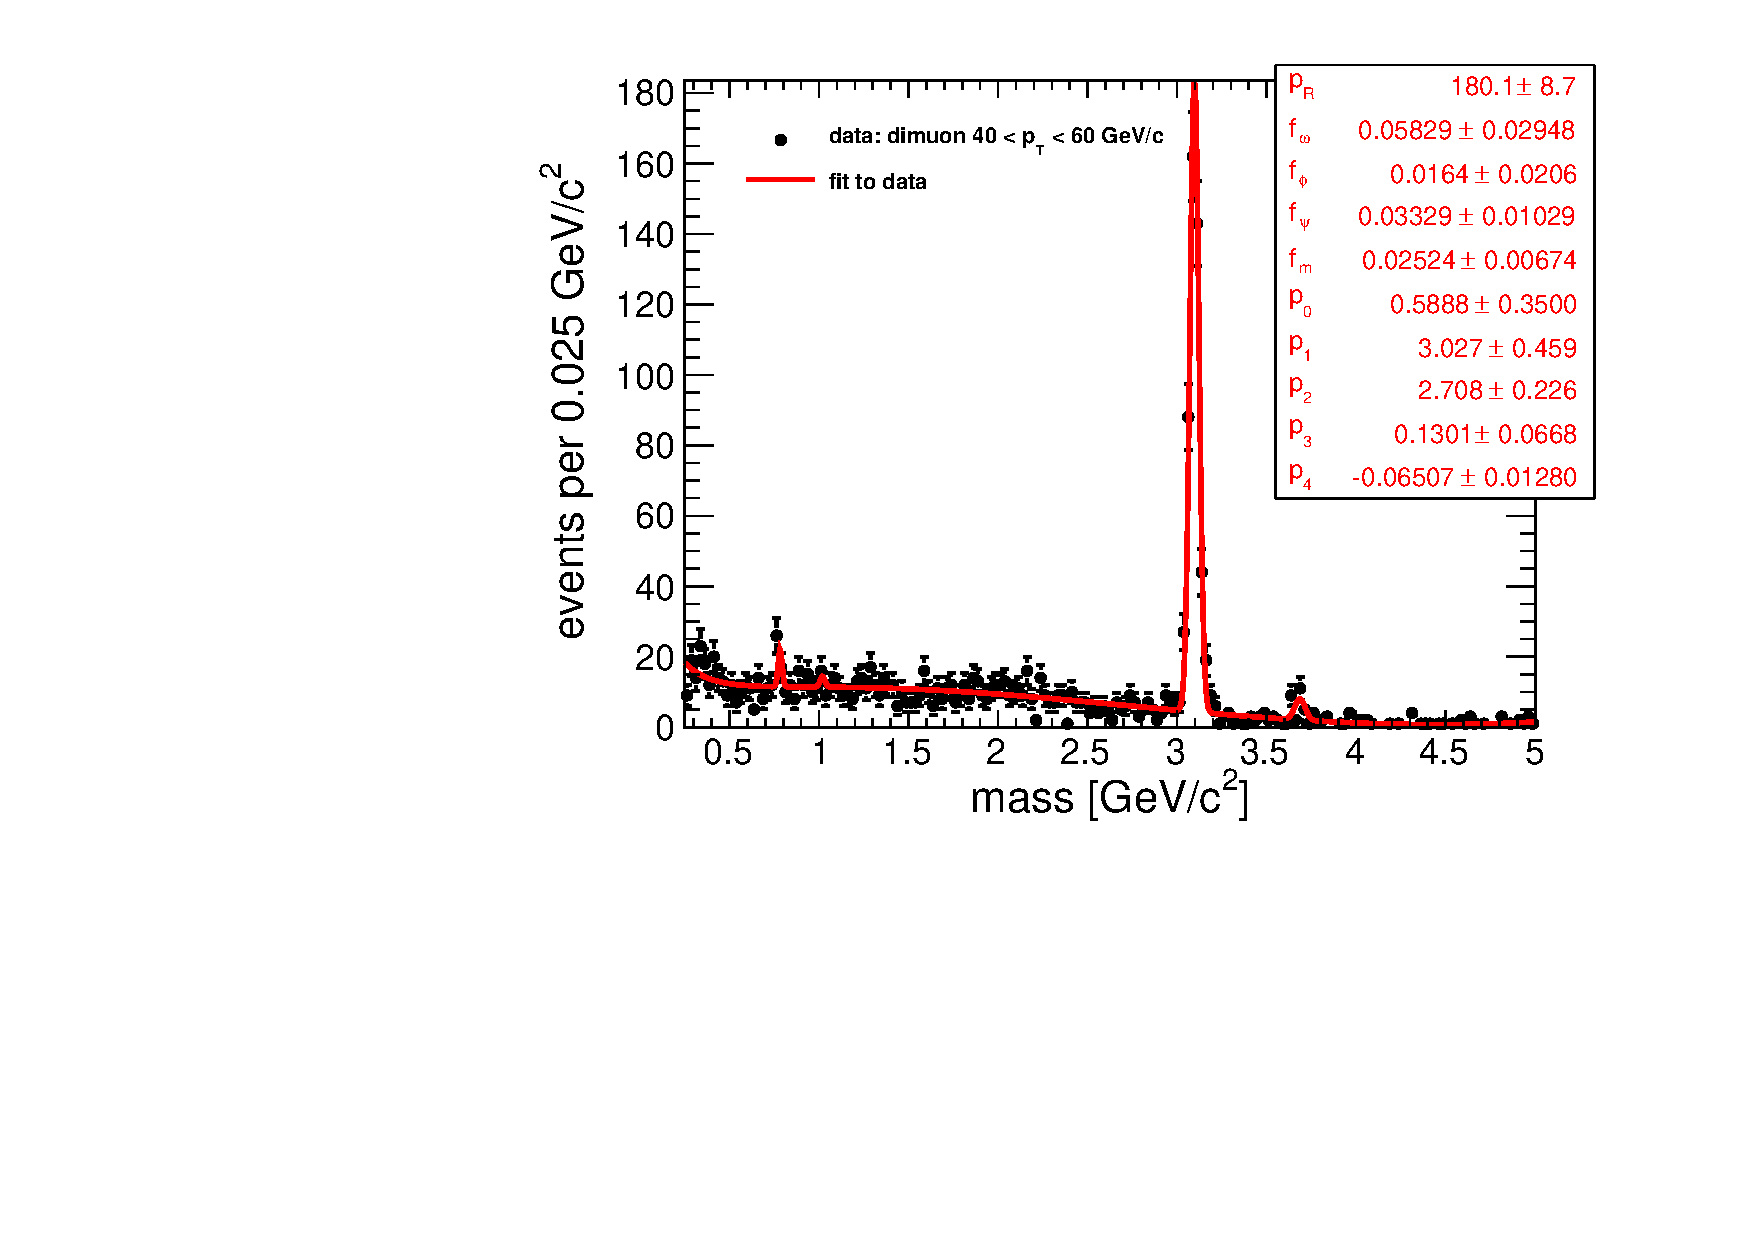
\includegraphics[width=\linewidth]{fullscale-backgroundEnriched_highpt.pdf}

\column{0.5\linewidth}
\centering control

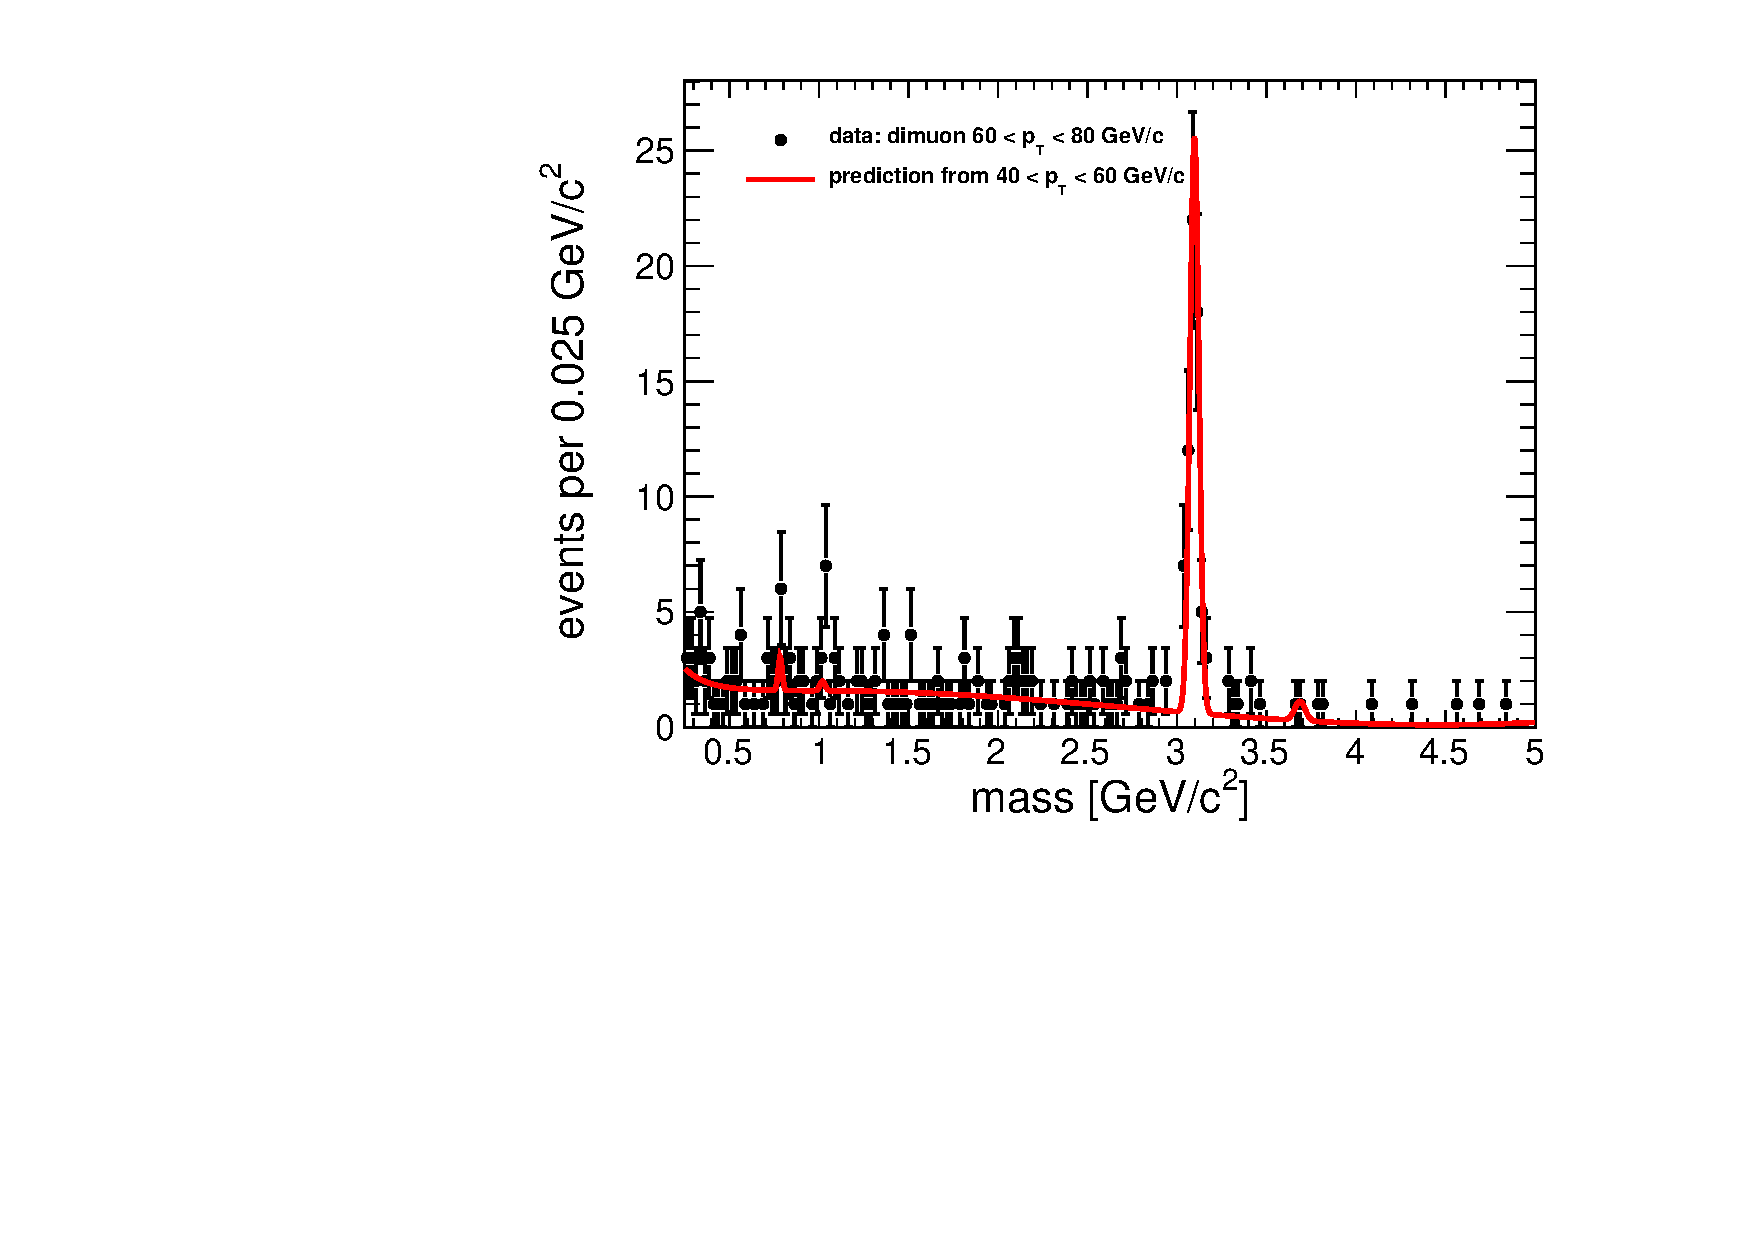
\includegraphics[width=\linewidth]{fullscale-control_highpt.pdf}
\end{columns}
\end{frame}

\begin{frame}
\frametitle{Region (a-2): high $\mu$ multiplicity}

\hfill 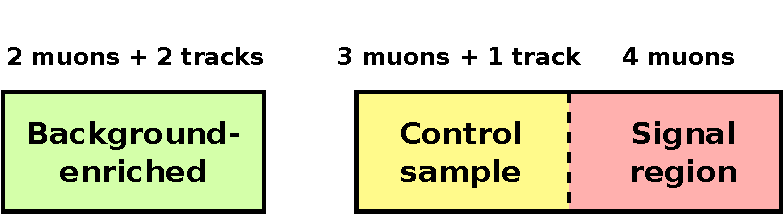
\includegraphics[width=0.5\linewidth]{bkgnd_control_signal_a-2.pdf}

\vspace{-1.5 cm}
\begin{itemize}
\item For the many-muons-in-one- \\ jet case, get the background \\ shape by adding tracks as \\ though they were fake muons
\item Resonances are dwarfed by a low-mass rise
\item MC dimuons with a muon known to be fake or decay-in-flight at
  generator level \textcolor{blue}{(blue)} reproduces the same spectrum
\end{itemize}

\begin{columns}
\column{0.5\linewidth}
\centering background-enriched

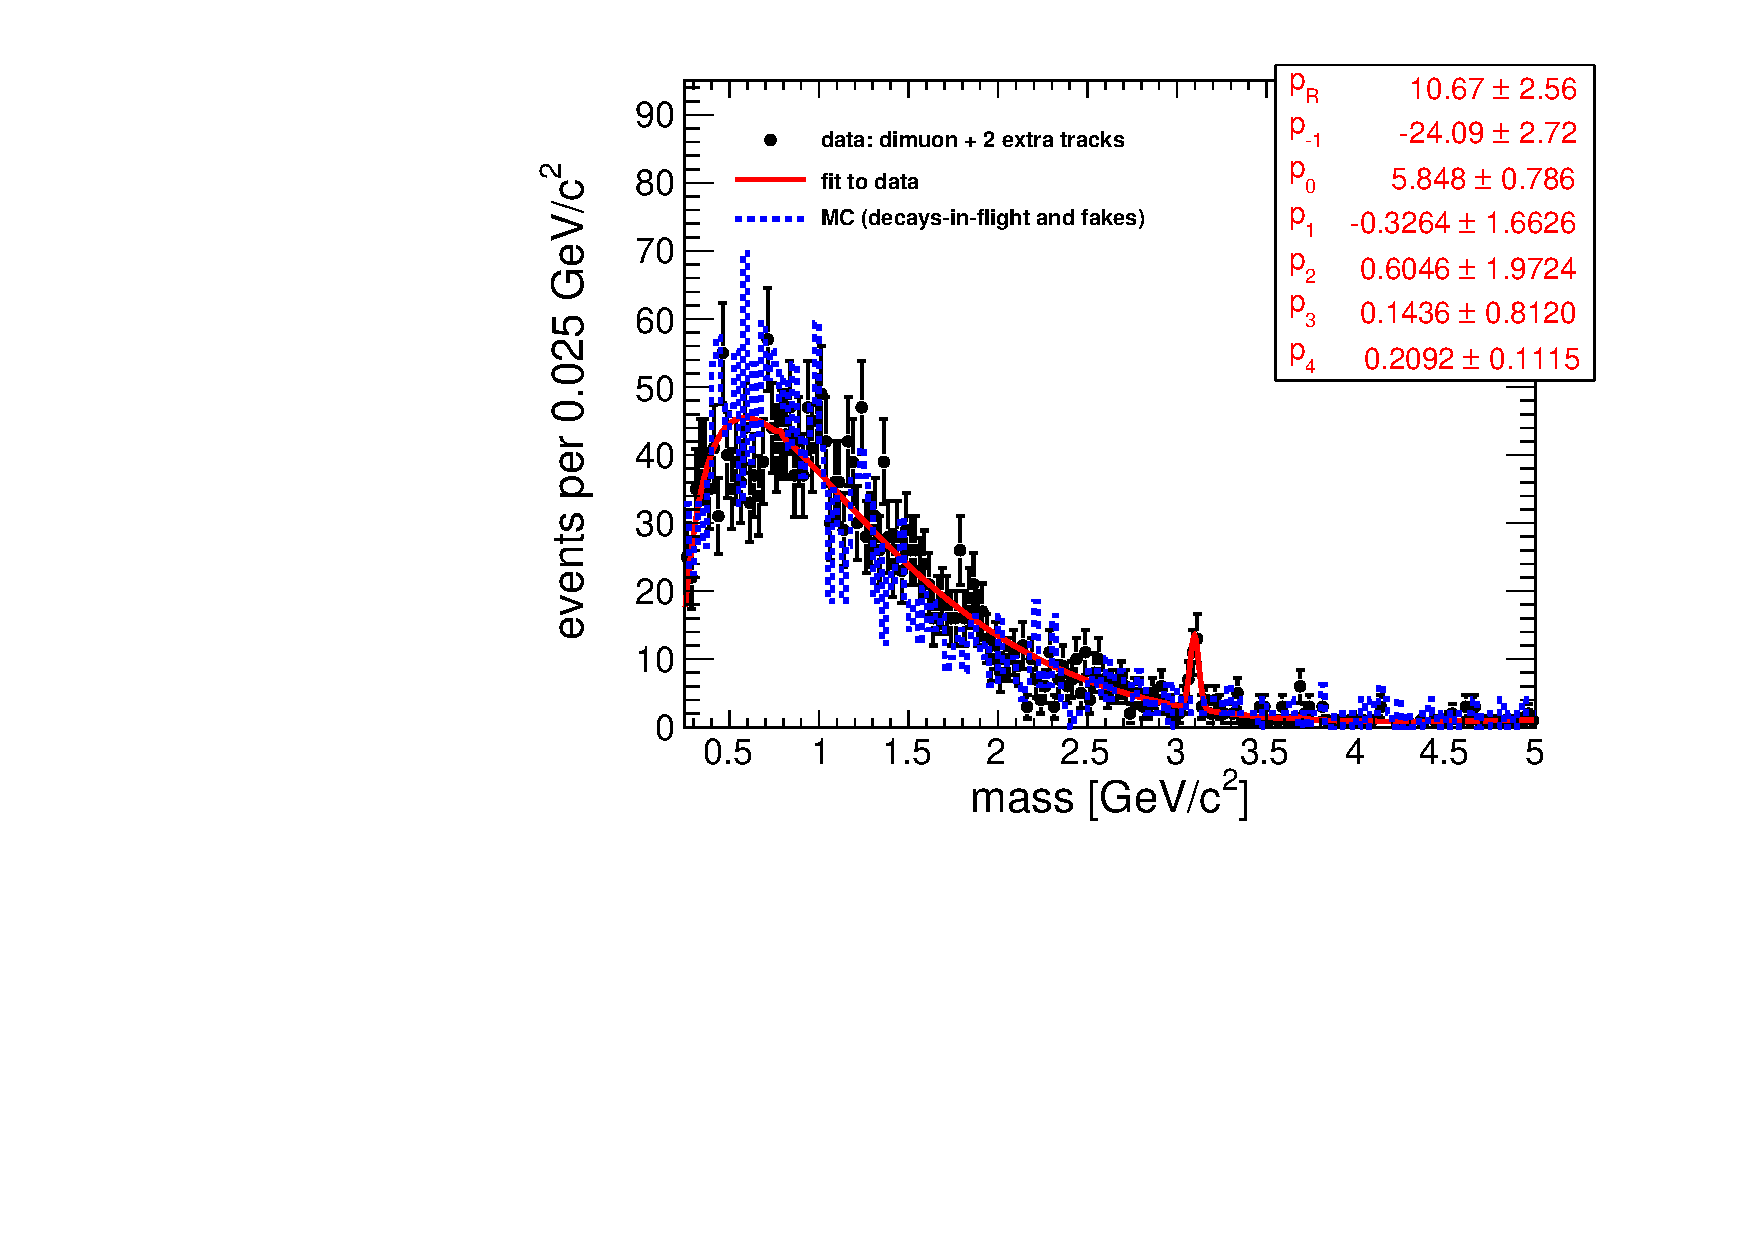
\includegraphics[width=\linewidth]{fullscale-backgroundEnriched_fakes.pdf}

\column{0.5\linewidth}
\centering control

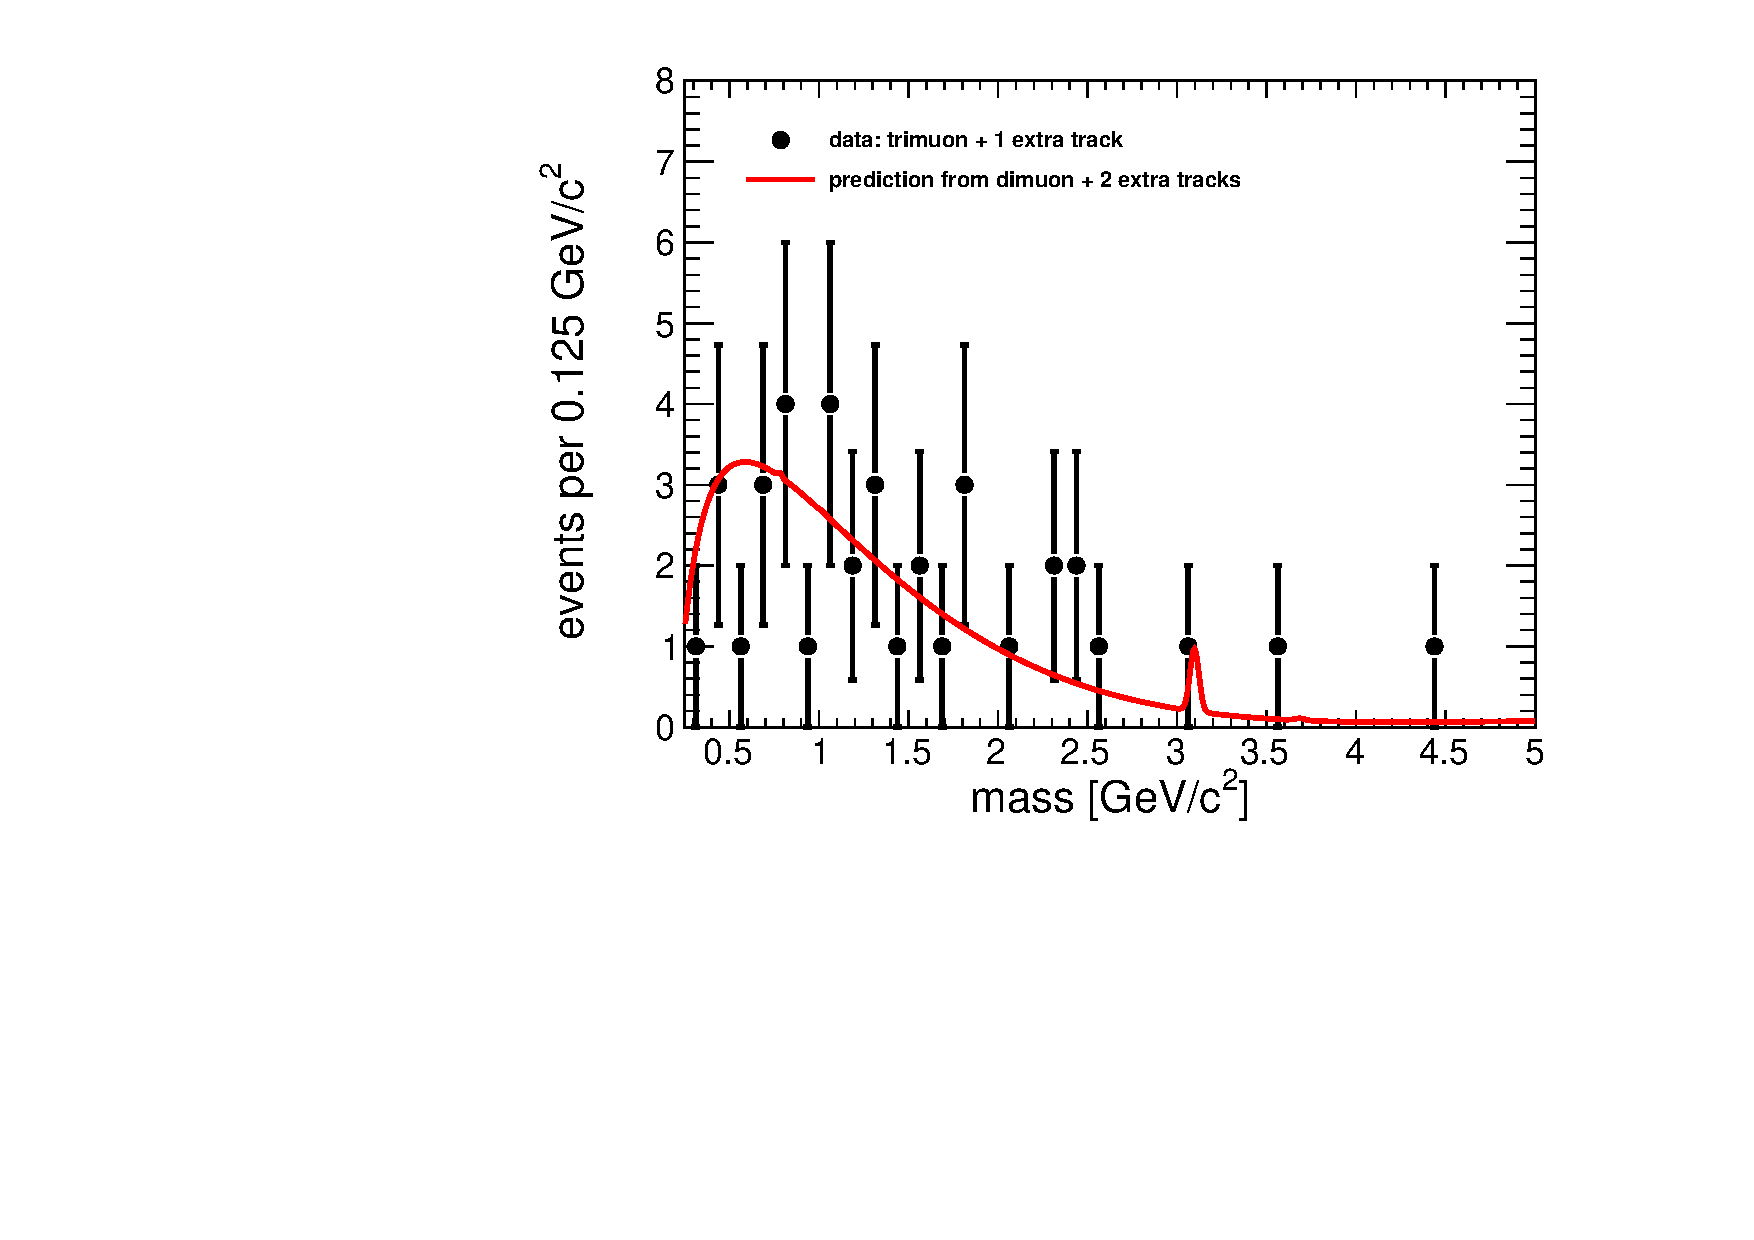
\includegraphics[width=\linewidth]{fullscale-control_fakes.pdf}
\end{columns}
\end{frame}

\begin{frame}
\frametitle{Region (b-1): two dimuons}

\hfill 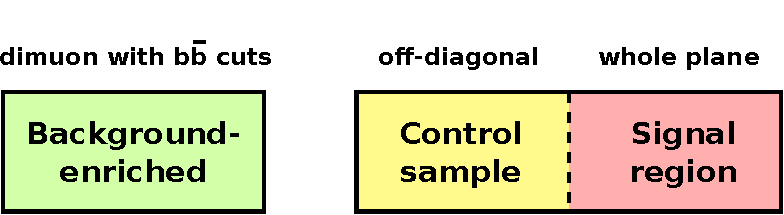
\includegraphics[width=0.5\linewidth]{bkgnd_control_signal_b-1.pdf}

\vspace{-1.5 cm}
\begin{itemize}
\item The only Standard Model \\ source that can give two \\ low-mass dimuons in the \\ same event is $b\bar{b}$ with both $b \to \mu\mu X$
\item Technicality: dimuon required to trigger the event {\scriptsize ($p_T > 20$~GeV/$c$)} \\ has a
  different distribution than the other dimuon {\scriptsize ($p_T > 10$~GeV/$c$)}
\begin{itemize}
\item background-enriched (triggered): apply the $b\bar{b}$ cuts (page~\pageref{pag:bbcuts})
\item background-enriched (other): request a third muon (from the other $b$-quark) to satisfy the trigger
\end{itemize}
\end{itemize}

\begin{columns}
\column{0.5\linewidth}
\centering background-enriched (triggered)

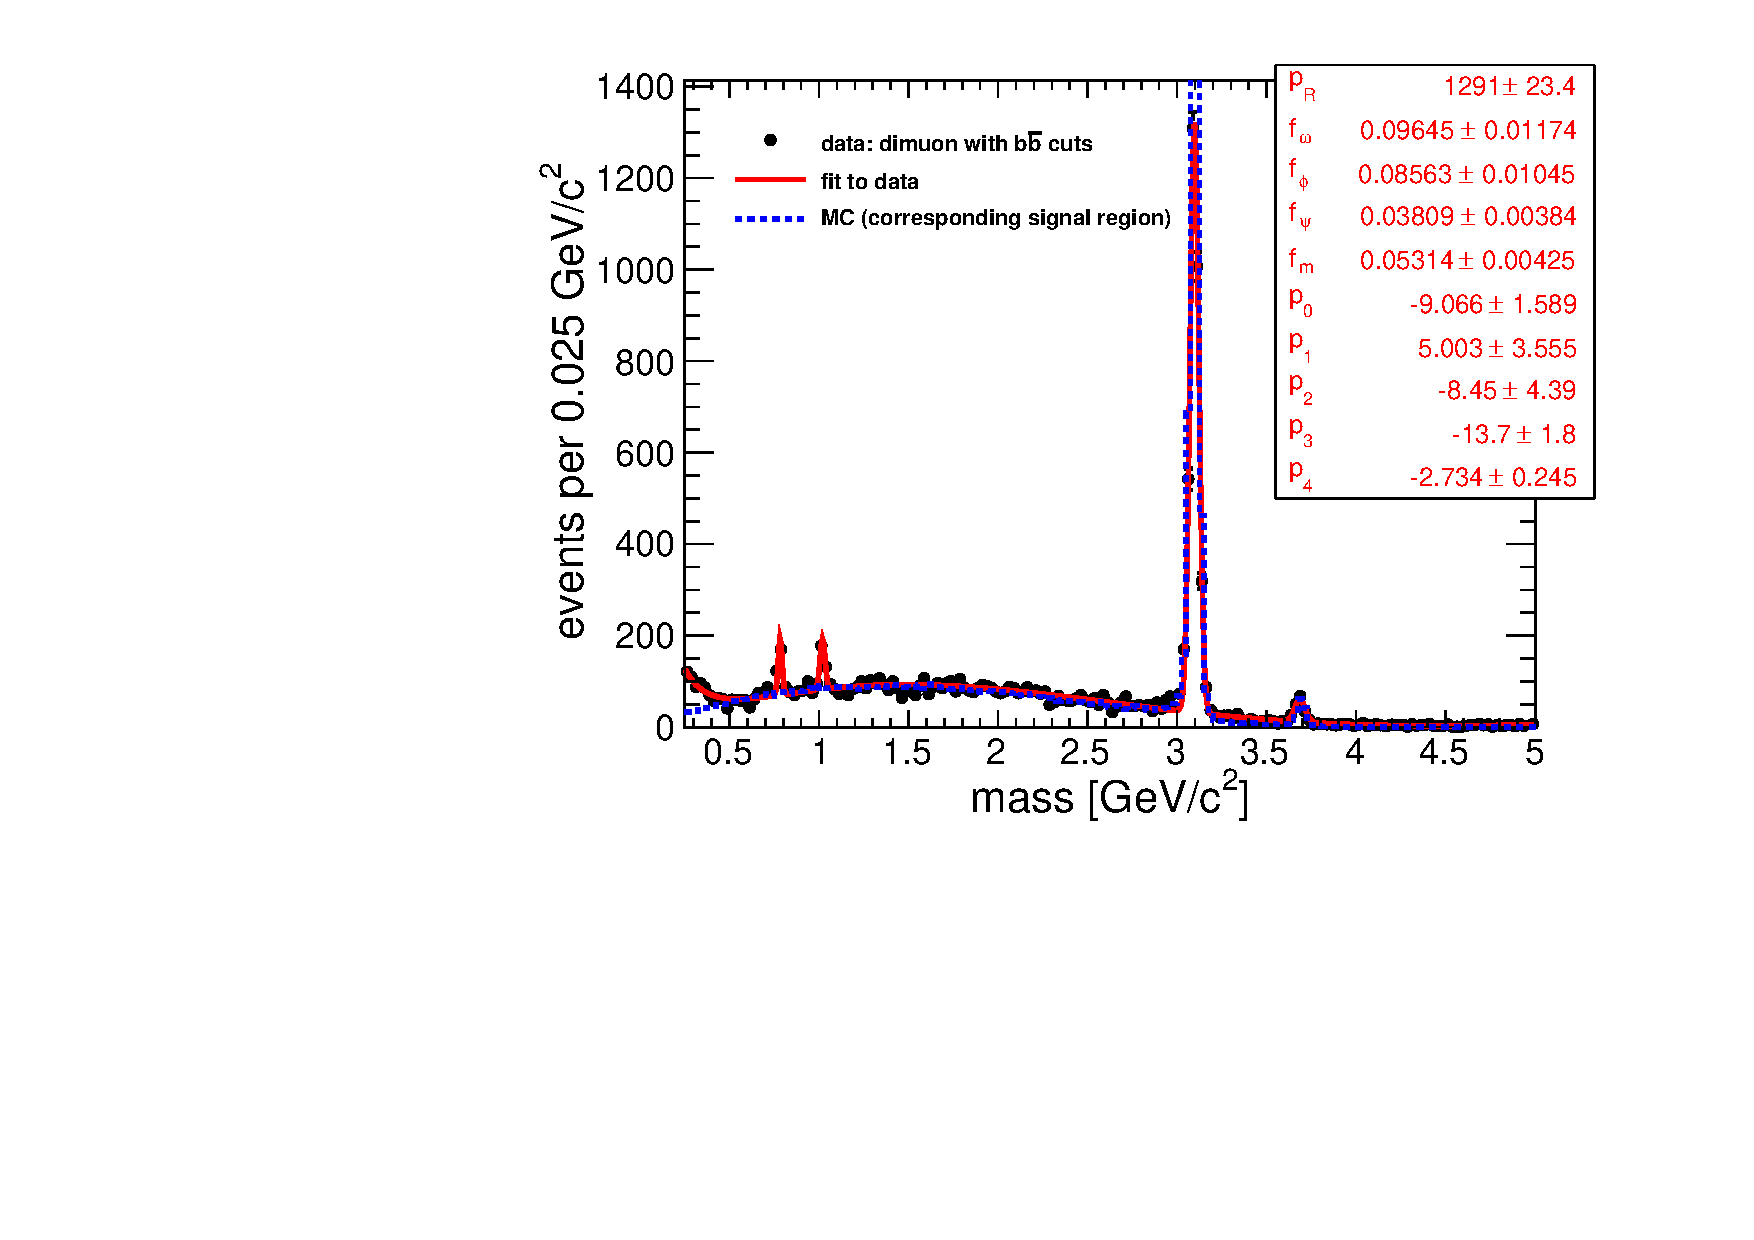
\includegraphics[width=\linewidth]{fullscale-backgroundEnriched_massC.pdf}

\column{0.5\linewidth}
\centering background-enriched (other)

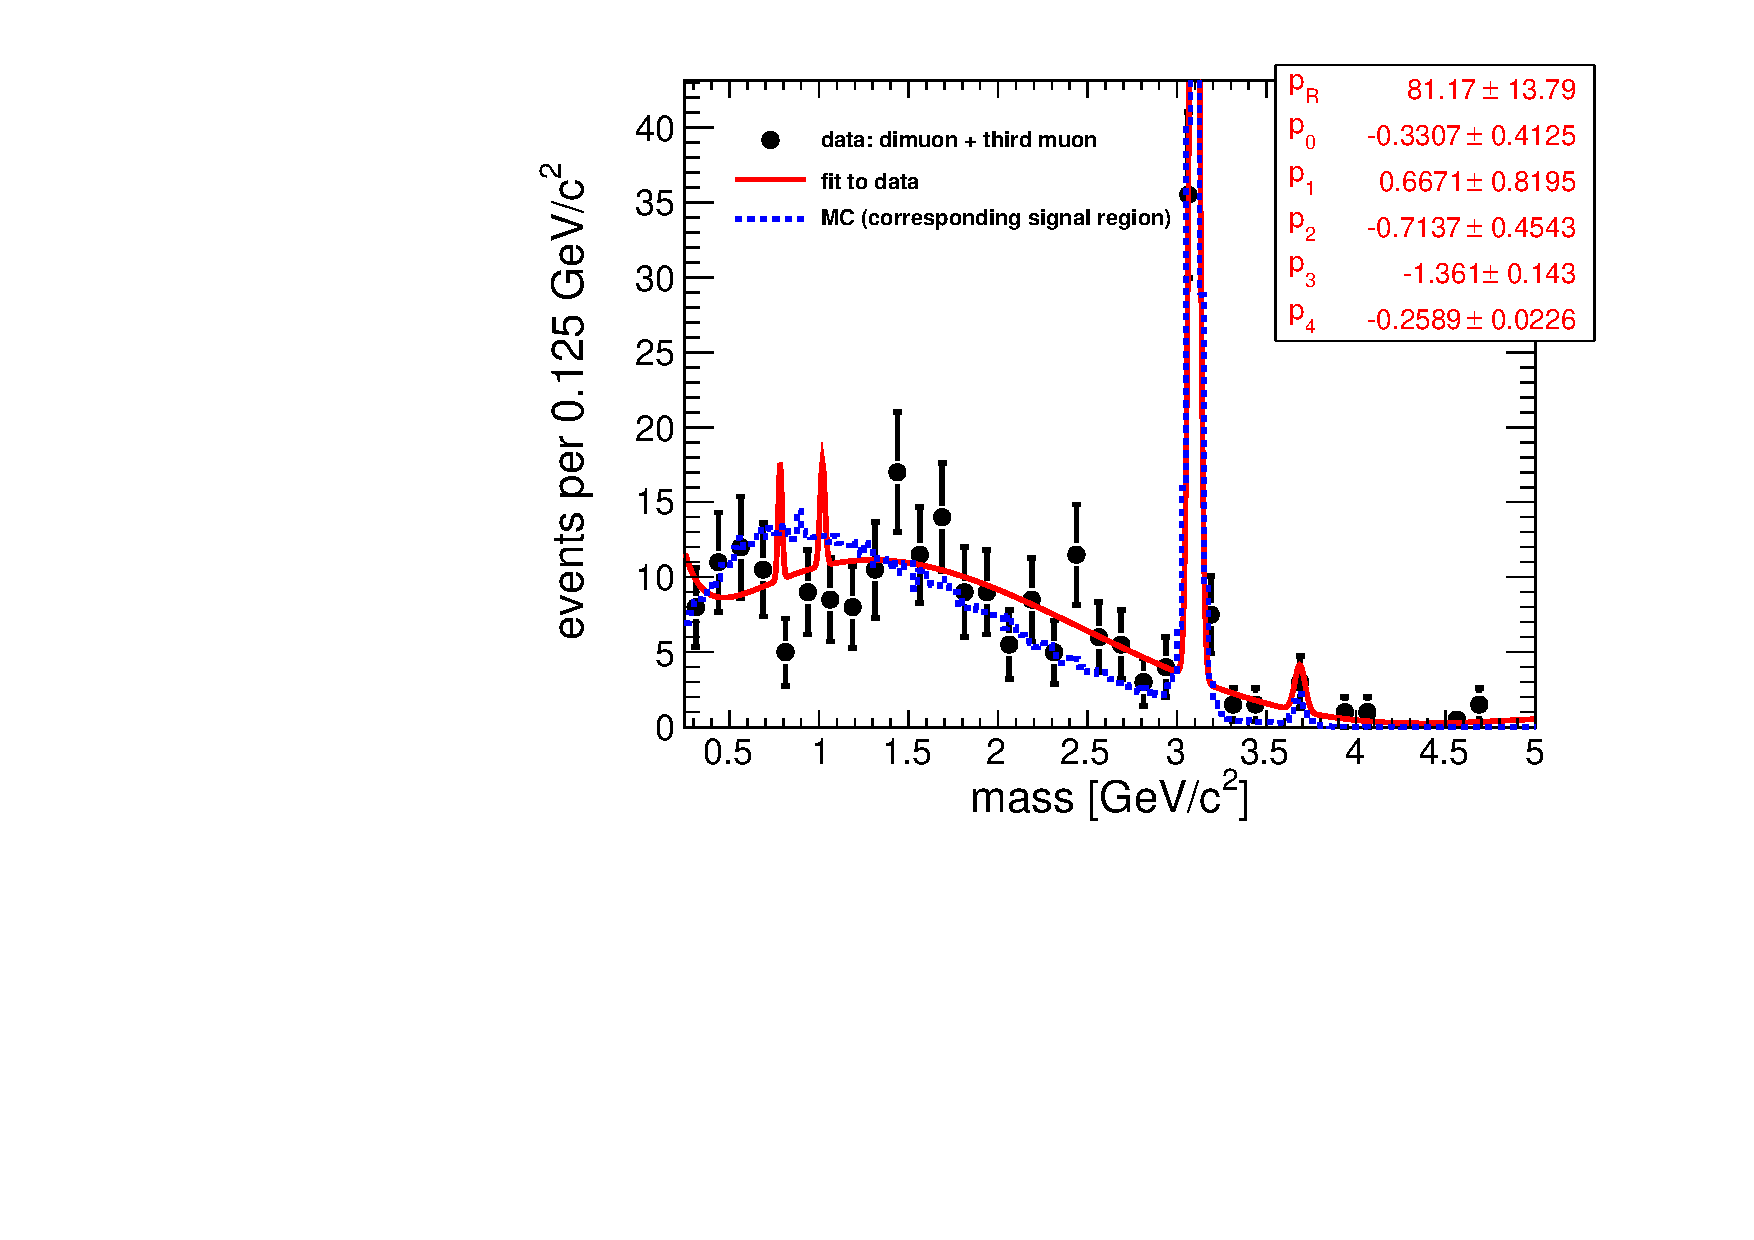
\includegraphics[width=\linewidth]{fullscale-backgroundEnriched_massF.pdf}
\end{columns}
\end{frame}

\begin{frame}
\frametitle{Region (b-1): two dimuons}

\begin{itemize}
\item Control region is the off-diagonal part of the mass-mass plane
\item Number of observed events is consistent with
  back-of-the-envelope scaling (0.2\% of $b$-quarks produce two
  $p_T > 5$~GeV/$c^2$ muons)
\item About 10\% of the background distribution is in the blinded region:
  observation of 10 events outside implies 1.1$\pm$0.4 inside
\end{itemize}

\vfill
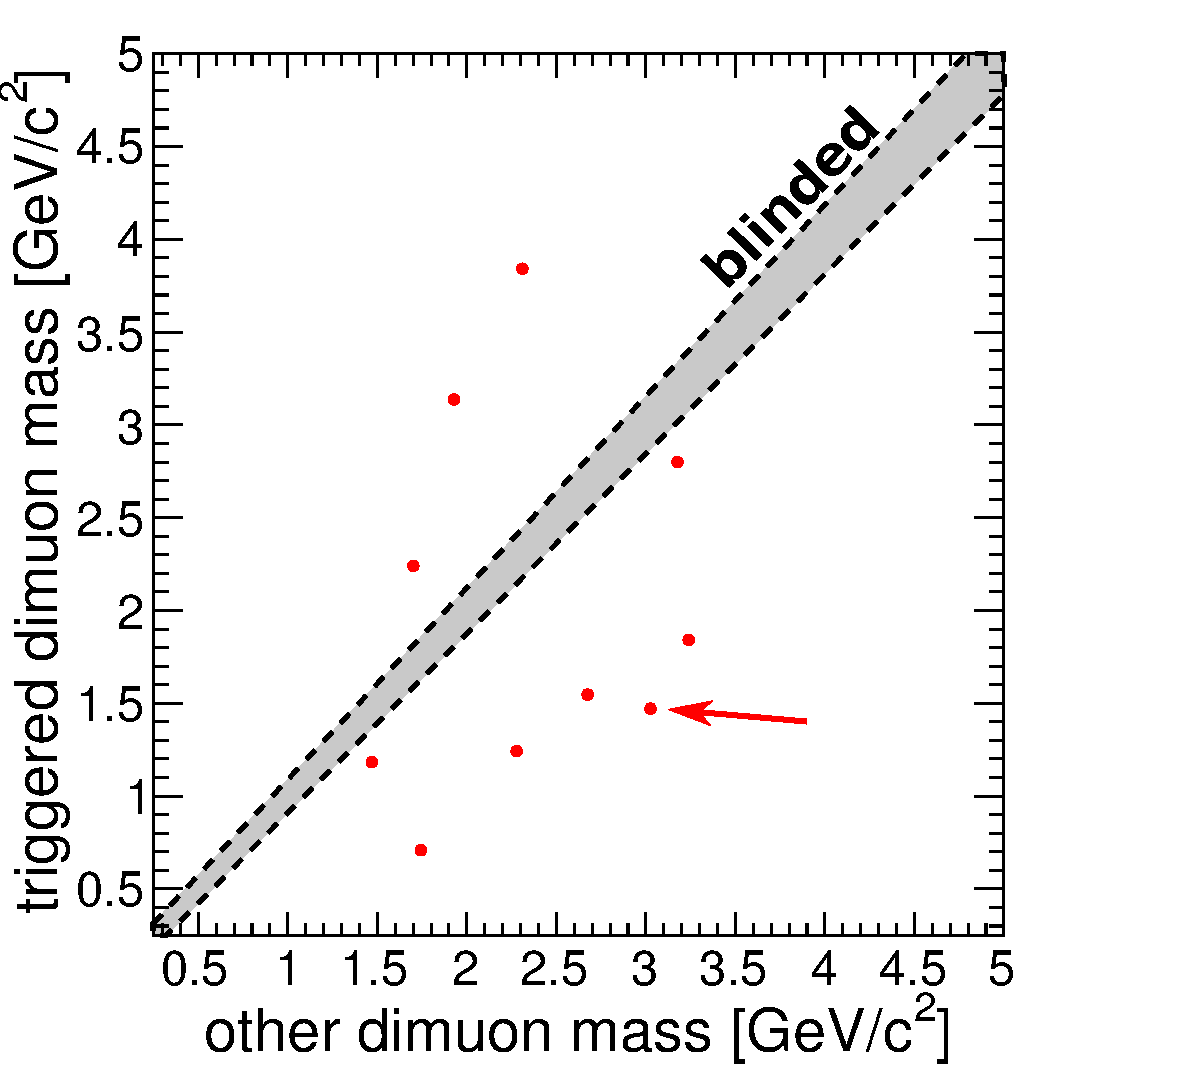
\includegraphics[height=4.9 cm]{data_dimudimu_wholecontrol.pdf} \hfill
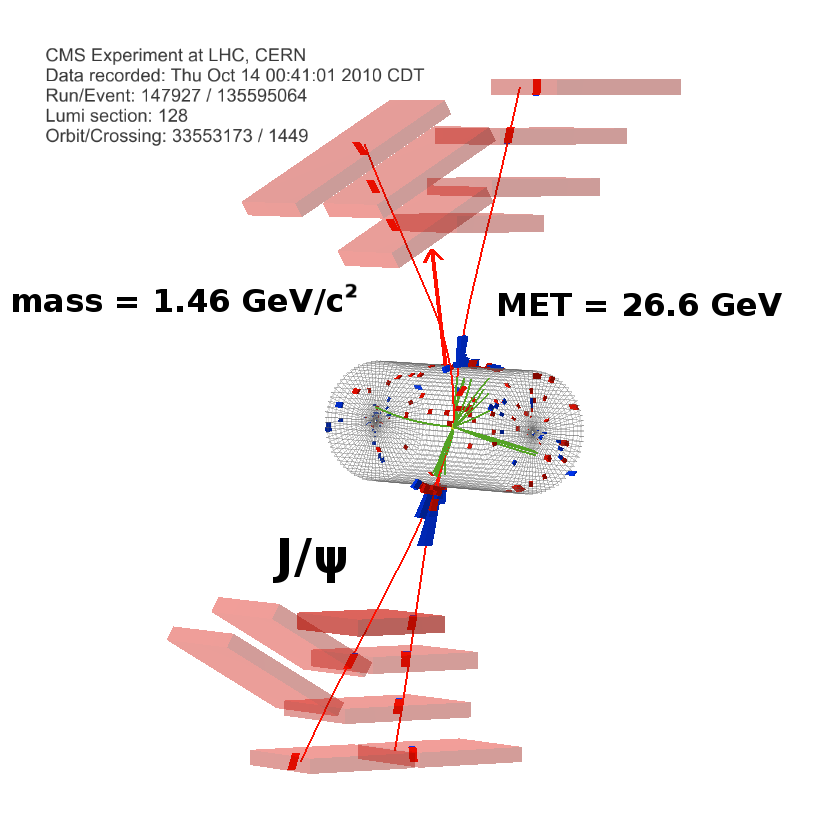
\includegraphics[height=4.9 cm]{dimudimu_control_eventdisplay.png}

\begin{itemize}
\item Control events all look like $J/\psi$ and double-semileptonic in $b\bar{b}$
\end{itemize}
\end{frame}

\begin{frame}
\frametitle{Signal shape systematics}

\begin{itemize}
\item Apart from the usual integrated luminosity and efficiency
  corrections, only important signal systematic is the resonance width
\item Resonance width is determined exclusively be detector resolution
  and muon final state radiation ($m_1$ decay width is small)
\item Measure detector resolution with $\omega$, $\phi$, $J/\psi$, and
  $\psi'$, then test high-$p_T$ dependence with Monte Carlo
\end{itemize}

\begin{columns}
\column{0.25\linewidth}
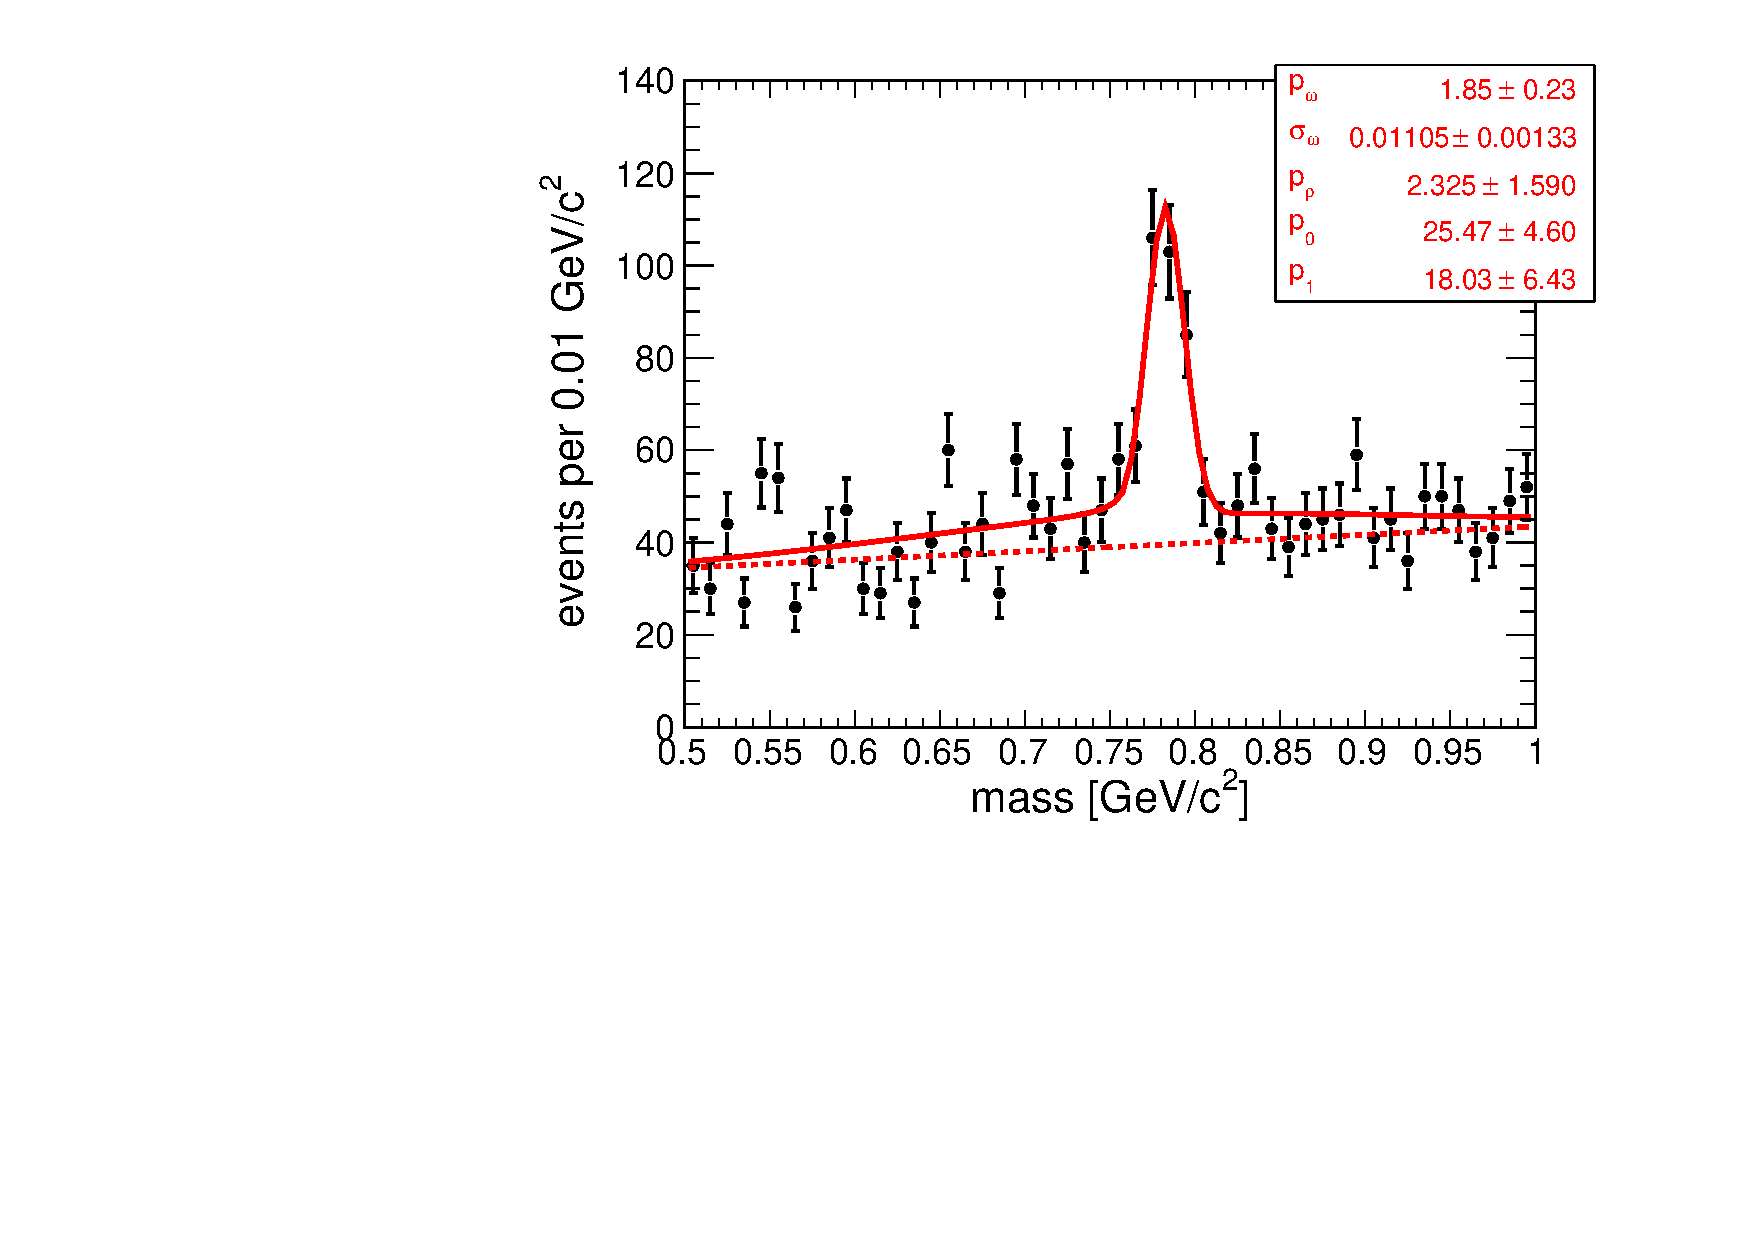
\includegraphics[width=\linewidth]{respeak_omega.pdf}

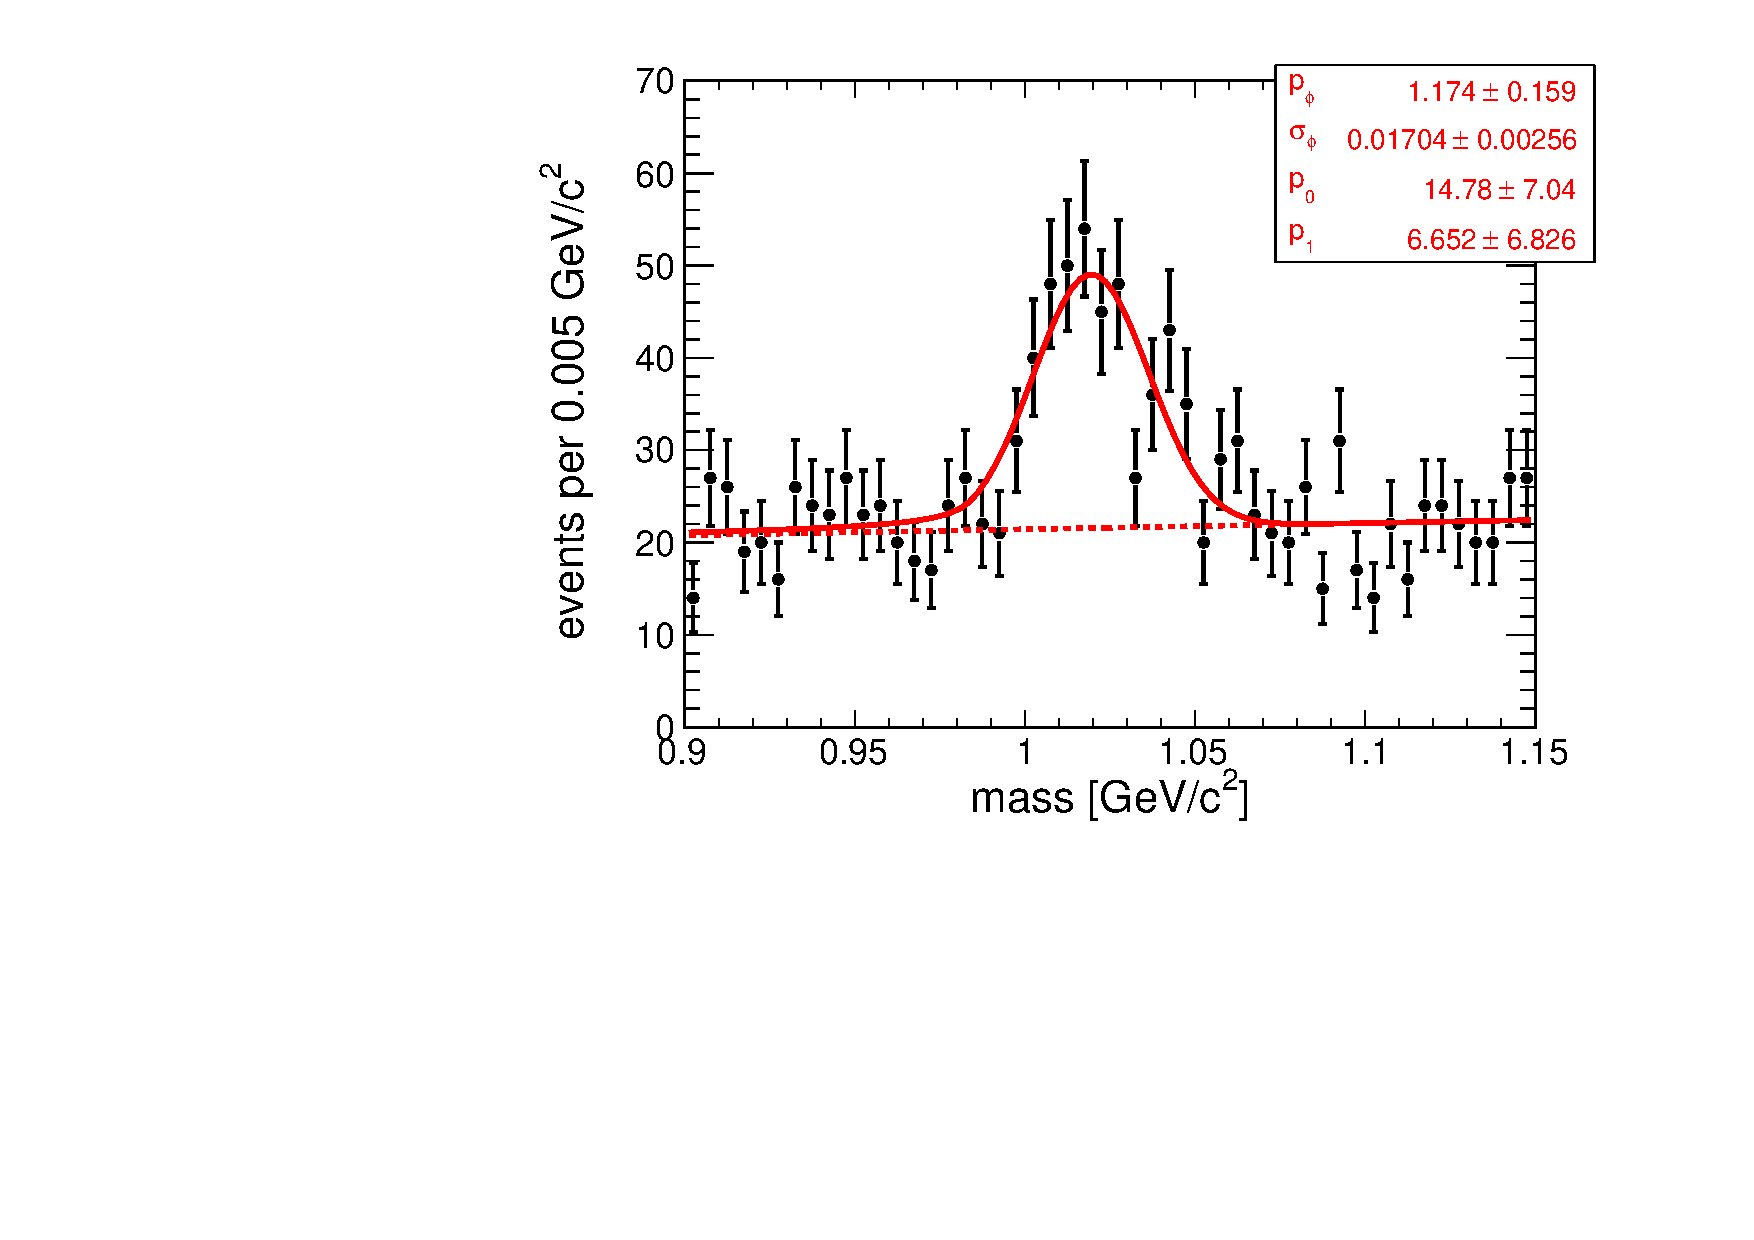
\includegraphics[width=\linewidth]{respeak_phi.pdf}

\column{0.25\linewidth}
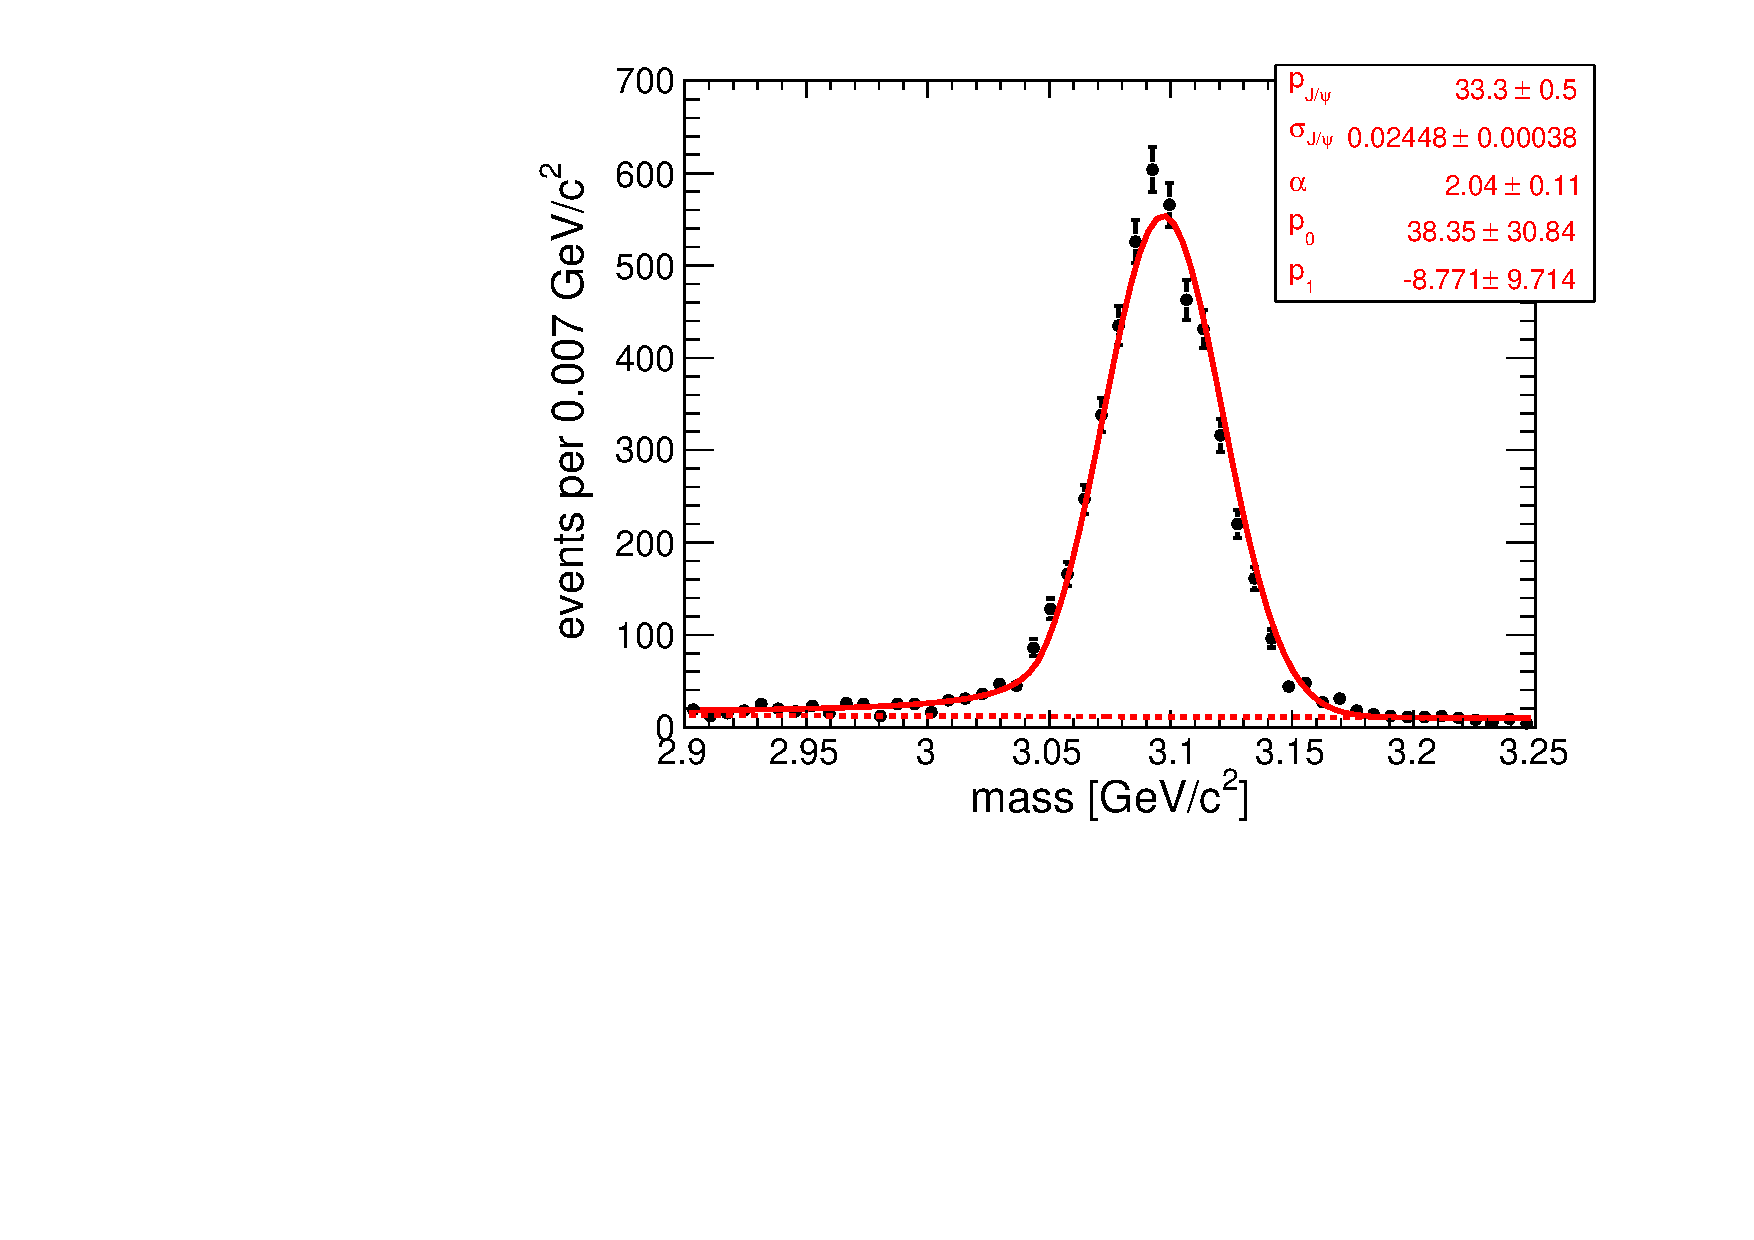
\includegraphics[width=\linewidth]{respeak_jpsi.pdf}

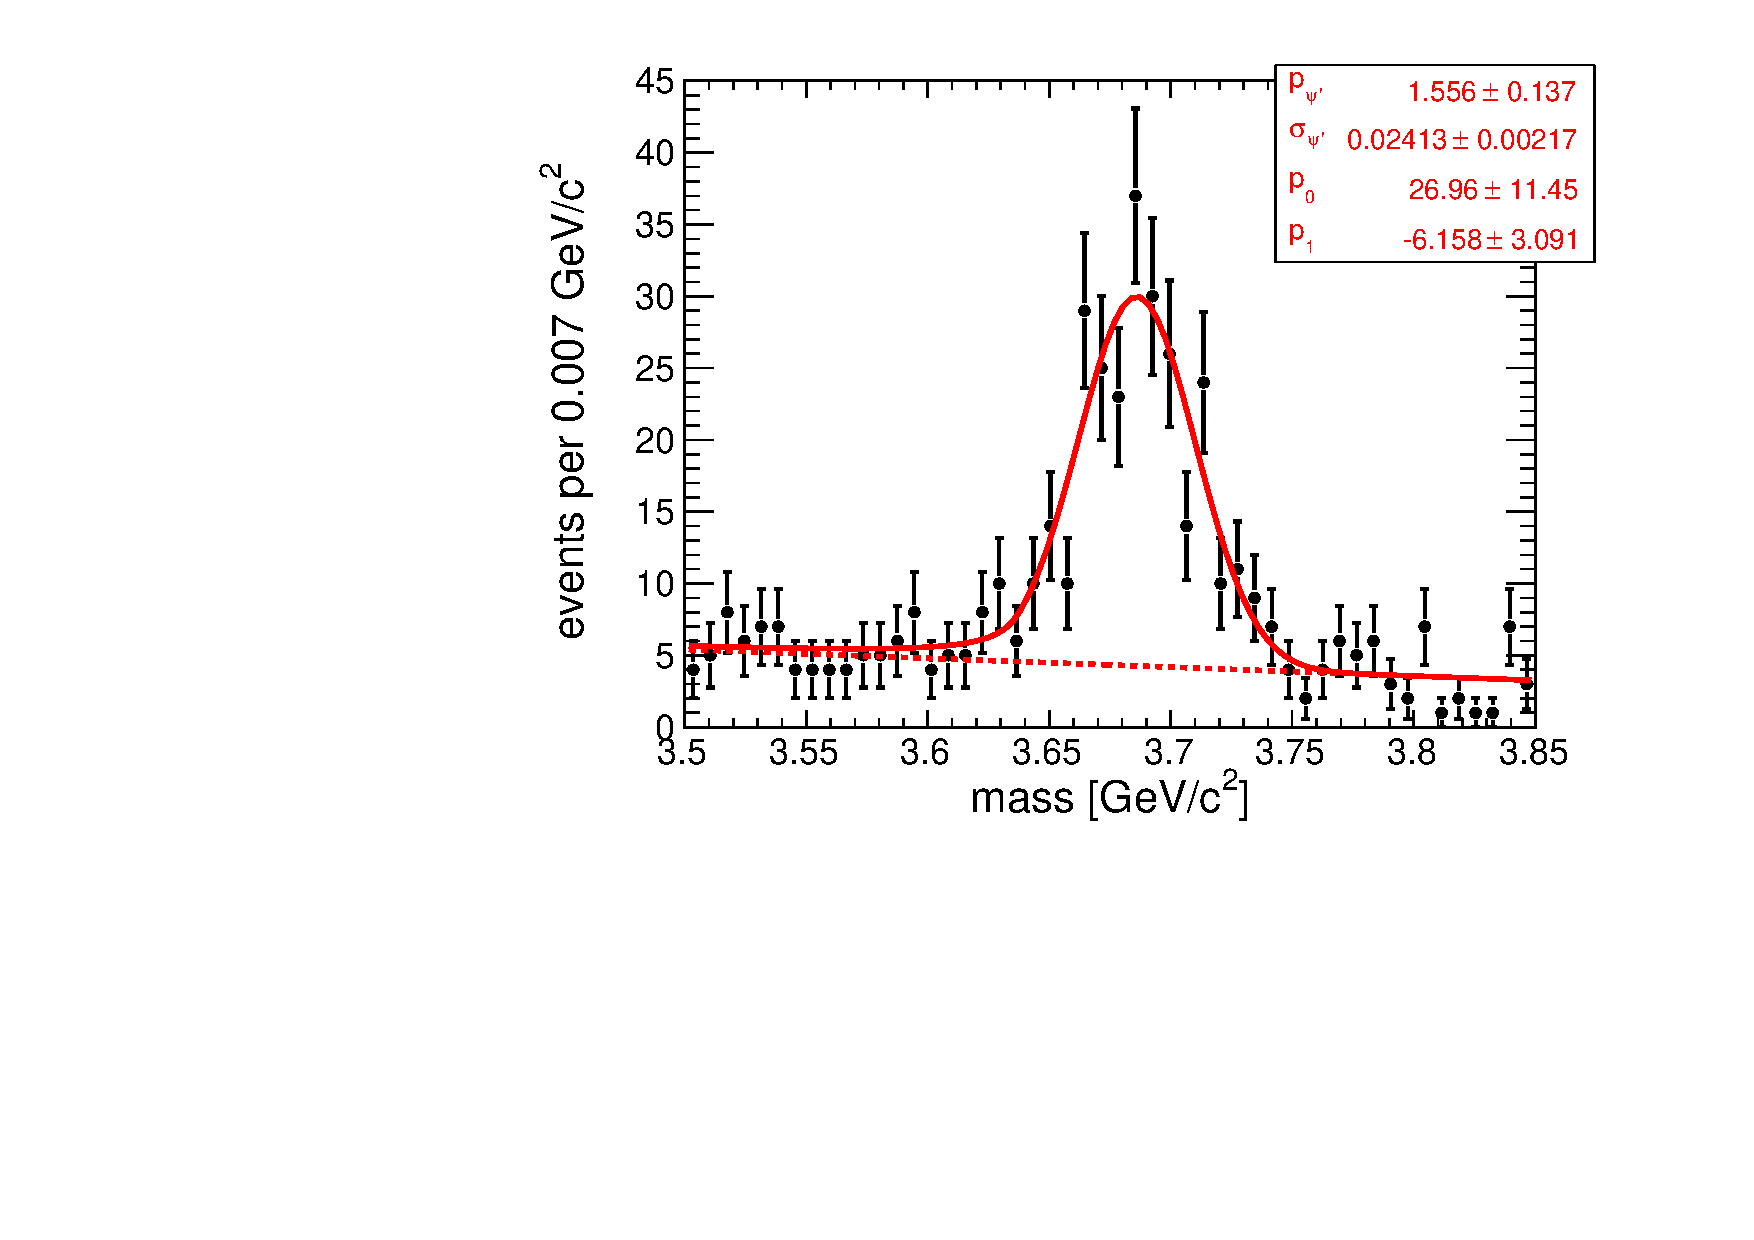
\includegraphics[width=\linewidth]{respeak_psiprime.pdf}

\column{0.5\linewidth}

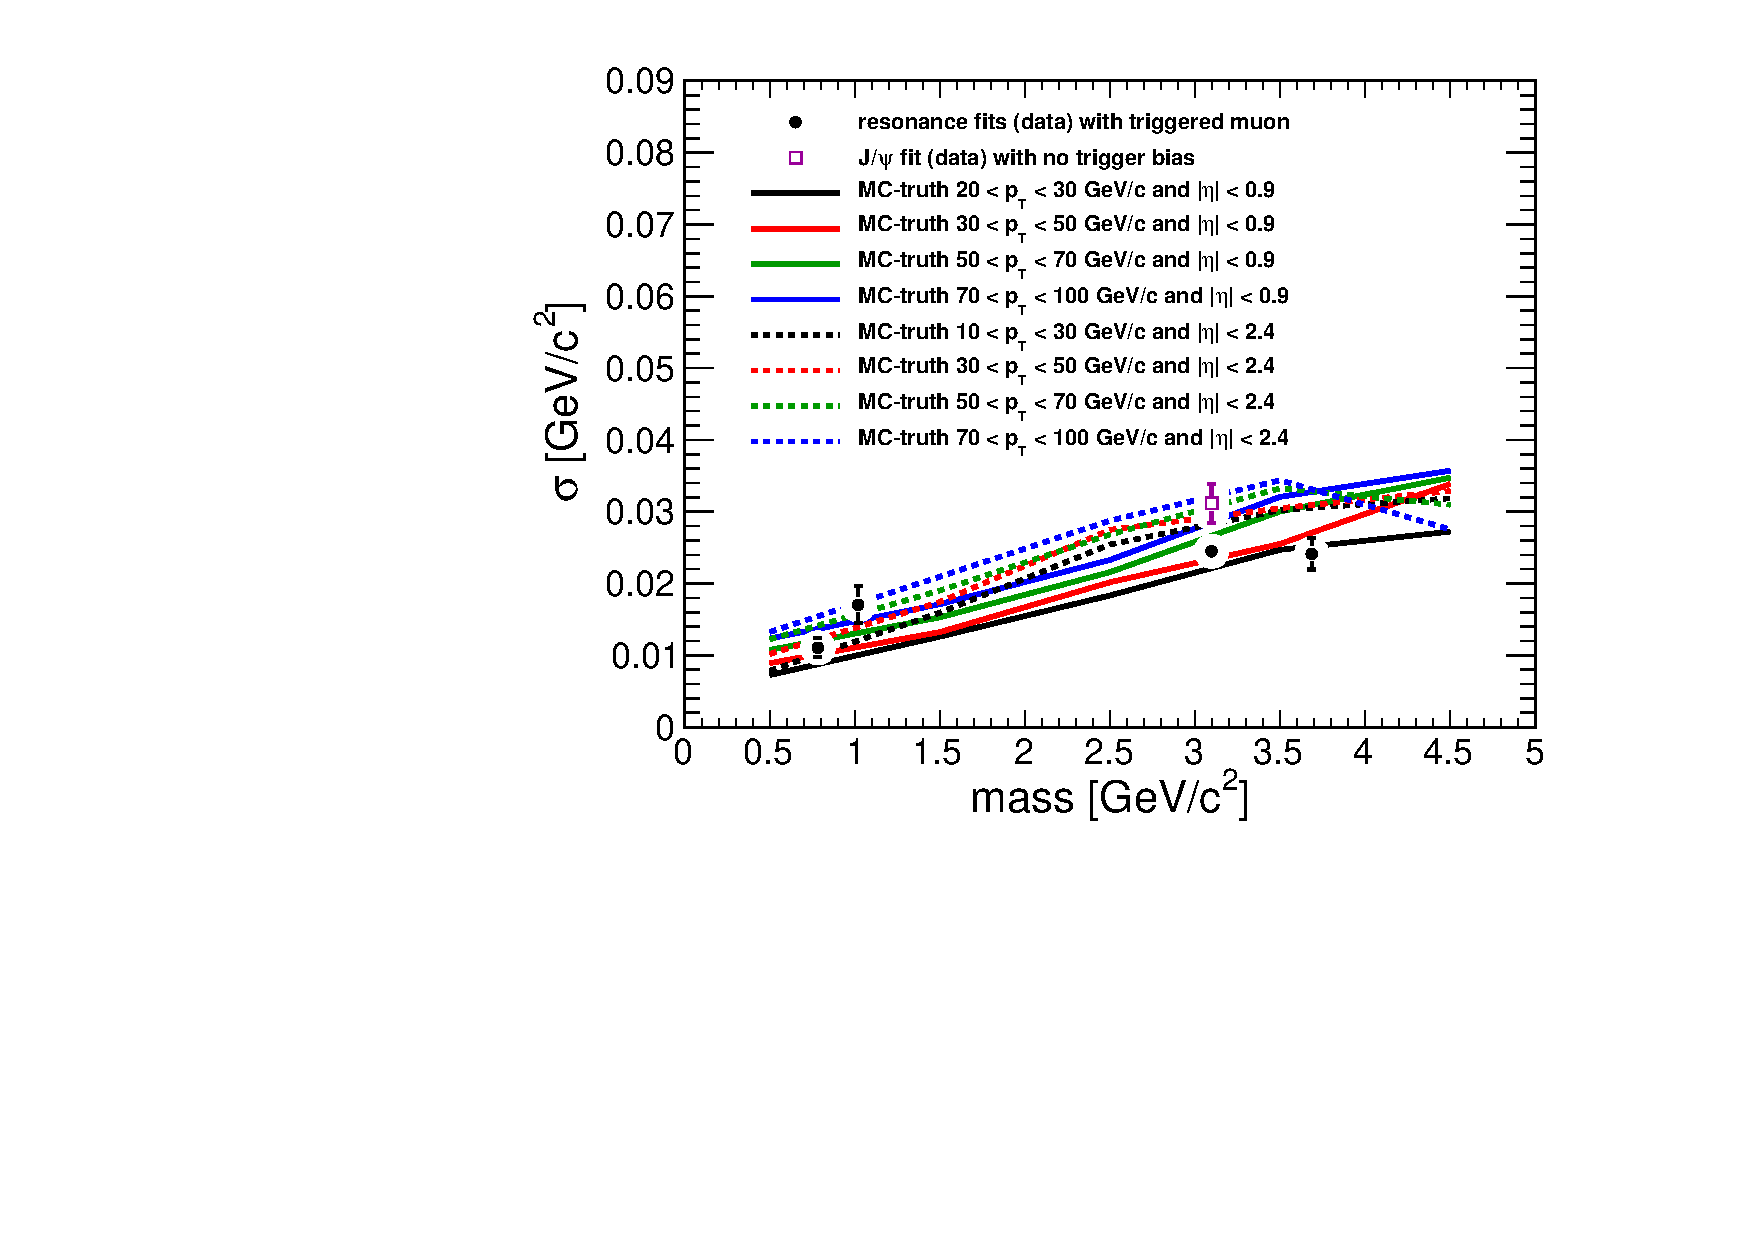
\includegraphics[width=\linewidth]{resolution.pdf}
\end{columns}

\begin{itemize}
\item Nice agreement, minimal dependence on $p_T$: signal shape is well-understood
\end{itemize}
\end{frame}

\section*{Fit results in control regions}
\begin{frame}
\begin{center}
\Huge \textcolor{blue}{Fit results in control regions}
\end{center}
\end{frame}

\begin{frame}
\frametitle{$n$-dimensional mass fitter}
\begin{itemize}
\item Sets upper limits on cross-section $\times$ branching fraction
  $\times$ acceptance as a function of $m_1$ resonance mass for each
  topology
\begin{itemize}
\item acceptance must be provided for a specific model
\end{itemize}

\item Implemented in RooFit/RooStats: using MCMC method with
  systematics modeled as log-normal distributions
\item Working values for systematic uncertainties (in progress):

{\scriptsize
\begin{tabular}{l l l}
Integrated luminosity & 11\% & \\
Efficiency & 5\% & estimate \\
Detector resolution & 27\% & from resonance fits \\
Template shape: $p_R$ (all resonances) & 10\% & \textcolor{darkblue}{(a-1)} background-enriched \\
Template shape: $f_\omega$ & 50\% & \textcolor{darkblue}{(a-1)} background-enriched \\
Template shape: $f_\phi$ & 125\% & \textcolor{darkblue}{(a-1)} background-enriched \\
Template shape: $f_{\psi'}$ & 30\% & \textcolor{darkblue}{(a-1)} background-enriched \\
\end{tabular}}

\item Currently a Gaussian signal shape: adding Crystal Ball tail

\item Test the full framework by calculating upper limits in the
  control regions, rather than the signal regions
\end{itemize}
\end{frame}

\begin{frame}
\frametitle{Testing the fitter in controls}

\begin{itemize}
\item The \textcolor{darkblue}{(a-1)} control region: single dimuon with $60 < p_T < 80$~GeV/$c$
\end{itemize}

\hspace{0.5 cm} 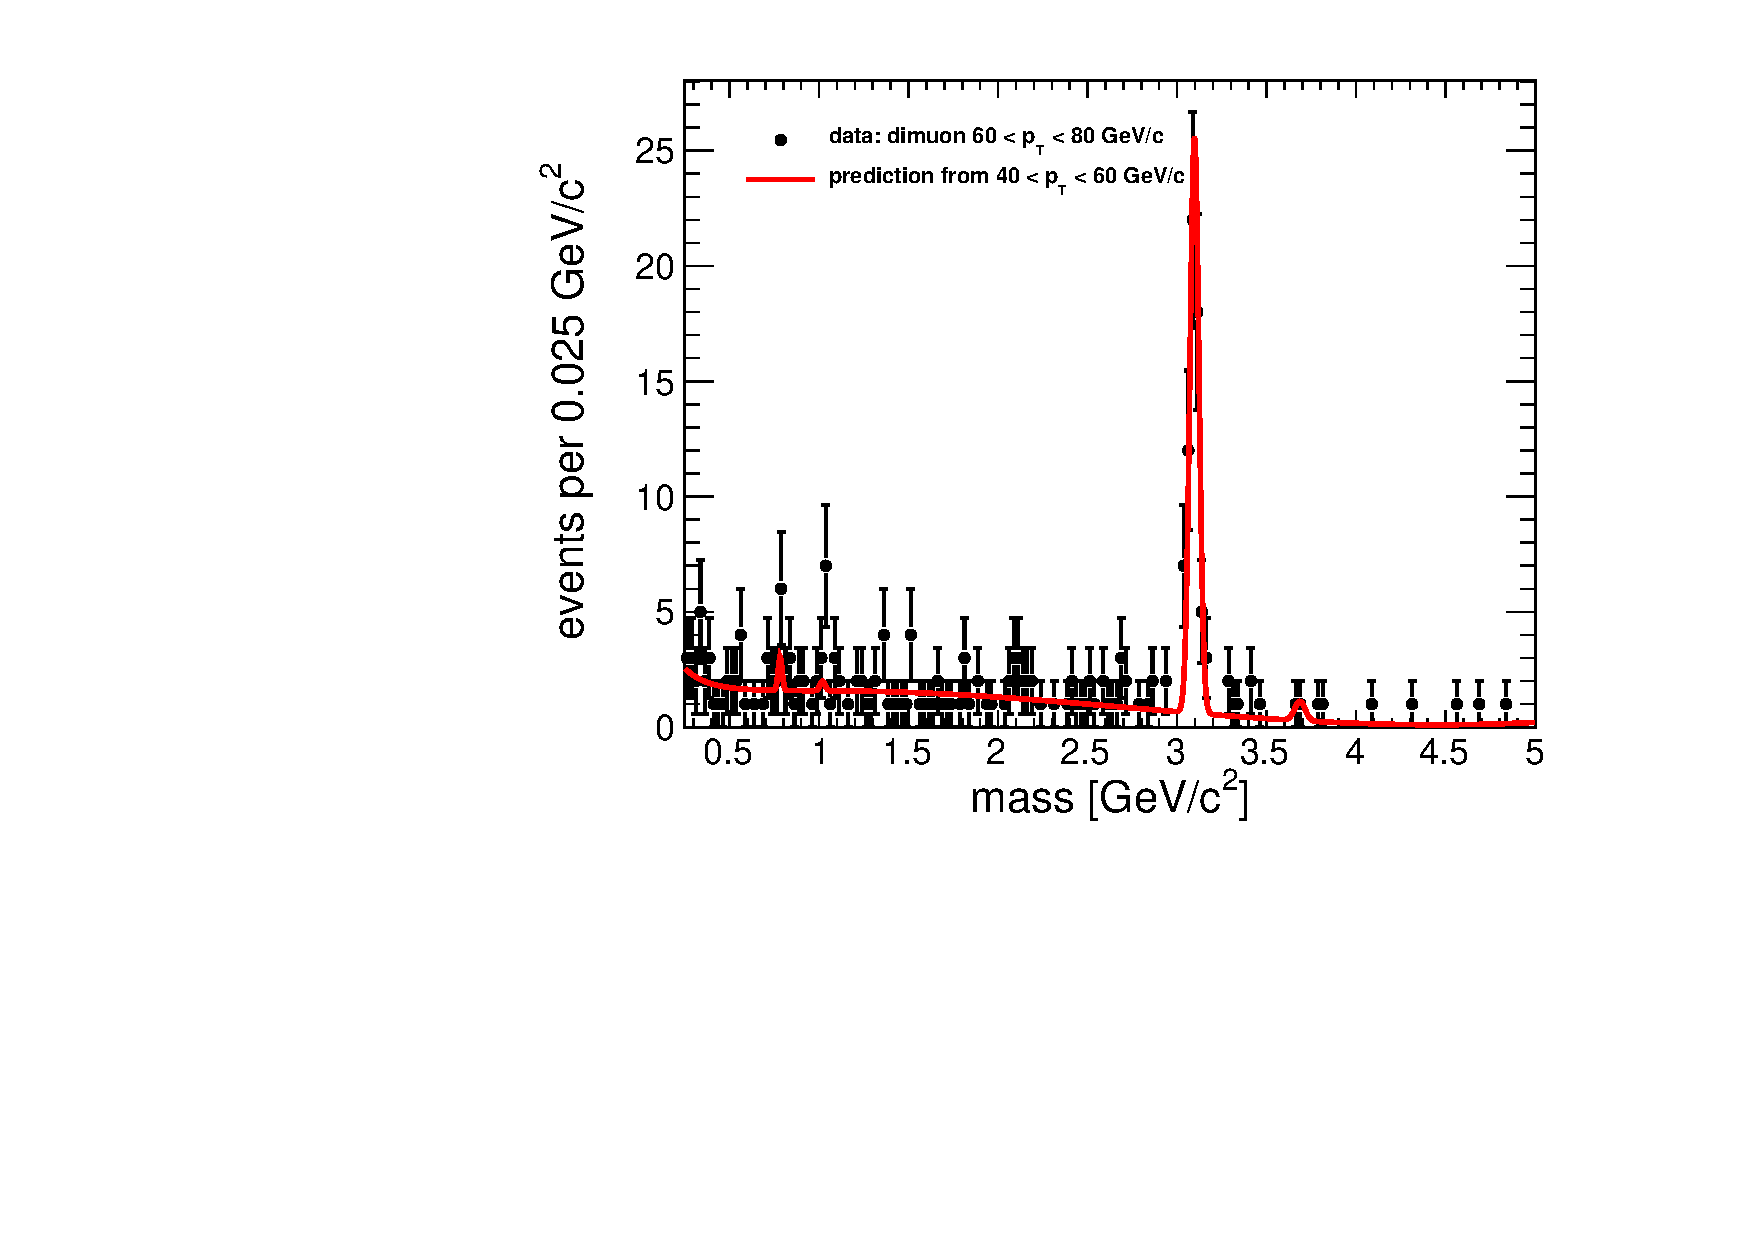
\includegraphics[height=3 cm]{fullscale-control_highpt.pdf} \hfill 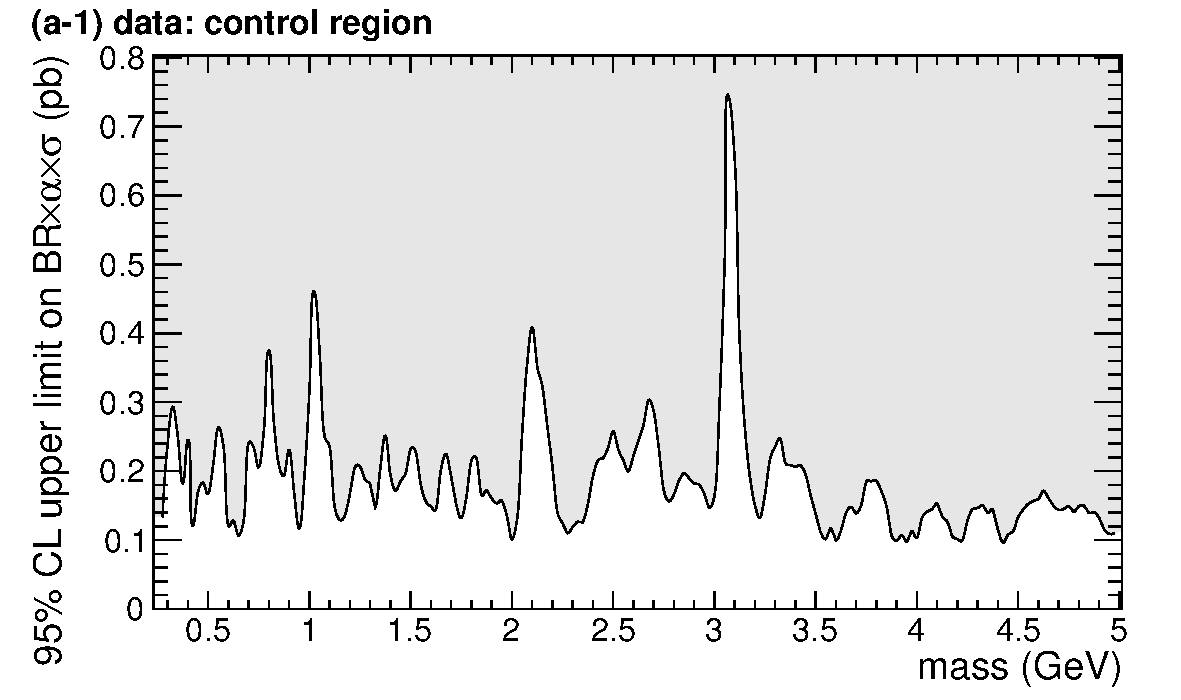
\includegraphics[height=3 cm]{ulimits_a-1.pdf} \hspace{0.5 cm}

\begin{itemize}
\item The \textcolor{darkblue}{(b-1)} control region: two dimuons per event, \mbox{$m_a \approx m_b$ blinded\hspace{-1 cm}}
\item The blinded region is modeled as containing zero events in this test
\end{itemize}

\hspace{0.5 cm} \hspace{0.75 cm} 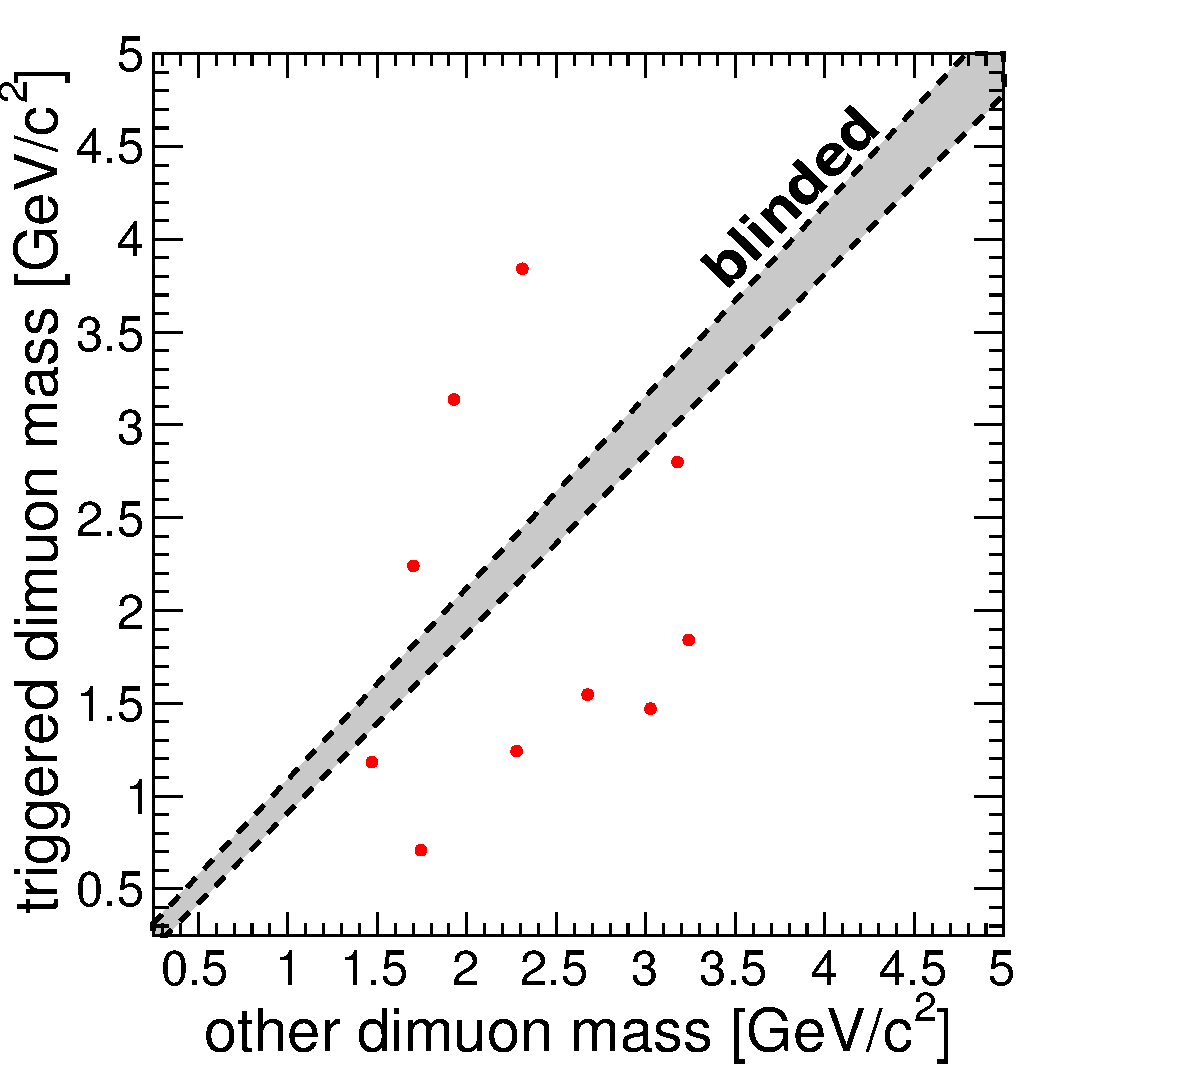
\includegraphics[height=3 cm]{data_dimudimu_wholecontrol_noarrow.pdf} \hfill 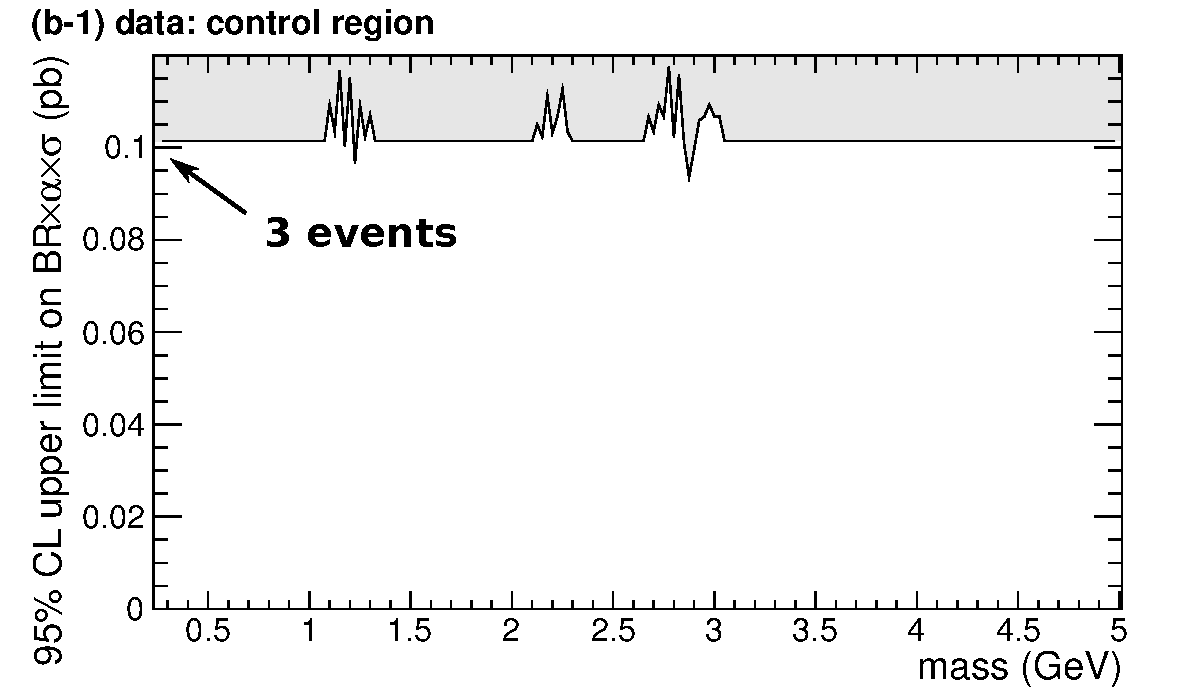
\includegraphics[height=3 cm]{ulimits_b-1.pdf} \hspace{0.5 cm}
\end{frame}

\section{Conclusions}

\begin{frame}
\frametitle{Conclusions}

\begin{itemize}\setlength{\itemsep}{0.5 cm}
\item ``Lepton jets'' are overlapping resonance decays with \mbox{well-defined mass\hspace{-1 cm}}

\item We search for a $\mu\mu$ mass peak using a signal + backgrounds
  fit, which provides a signal yield and background estimate at the
  same time, with the same data

\item Deriving the background-shape templates requires some care: select events by physics type to produce the right kinematics and test in control regions before using in the fit

\item The control regions are conforming to expectations, and the fitter is producing meaningful results

\item We'll be unblinding the signal soon
\end{itemize}

\label{numpages}
\end{frame}

\section*{Backup}
\begin{frame}
\begin{center}
\Huge \textcolor{blue}{Backup}
\end{center}
\end{frame}

\begin{frame}
\frametitle{Low-mass dimuons}

{\tiny Drell-Yan output from Pythia output, rather than $Z$-scaling.
  All plots range 0.25--5~GeV/$c^2$ in 190 bins.  ``Low-mass'' is
  0.35--0.5~GeV/$c^2$, ``continuum'' is 1.1--2.9~GeV/$c^2$.
  $b\bar{b}$ cuts are: $Iso > 4.5\mbox{ GeV/$c$}\mbox{ \bf or }L_{xy}
  > 2\mbox{ mm}$.}

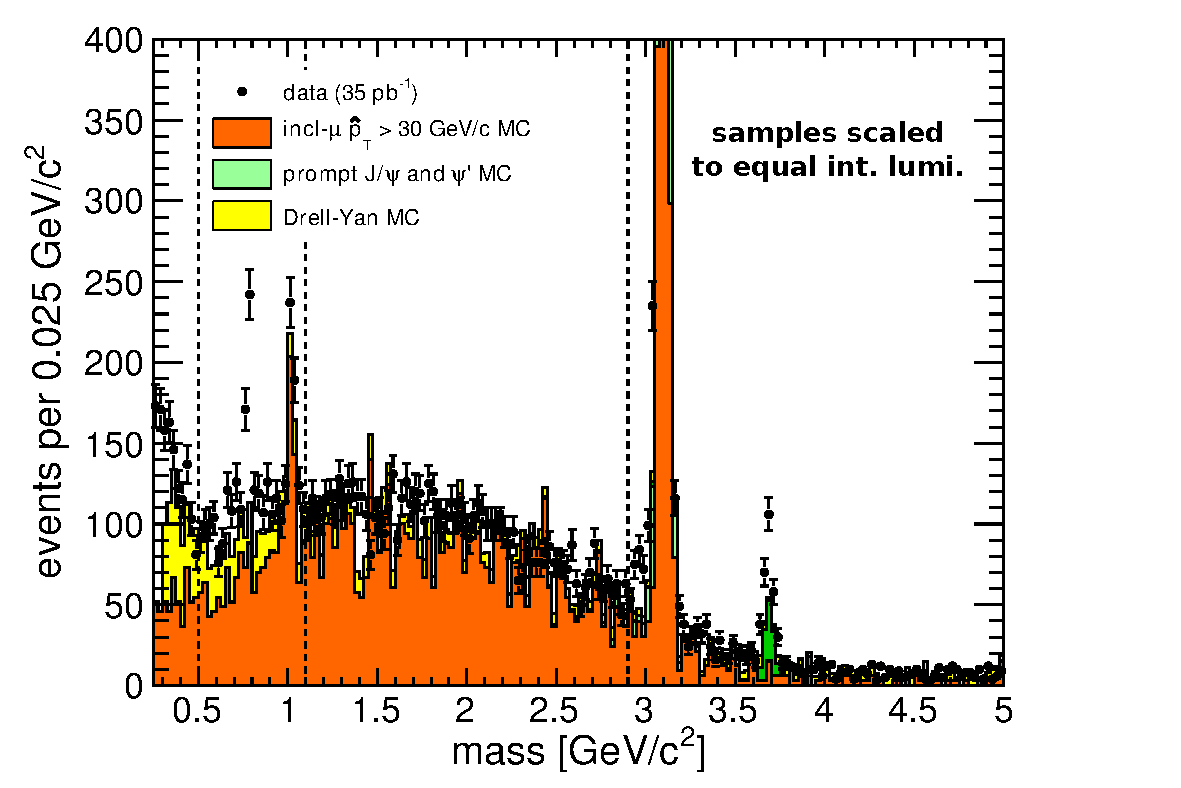
\includegraphics[width=0.33\linewidth]{support_mass_all.pdf}
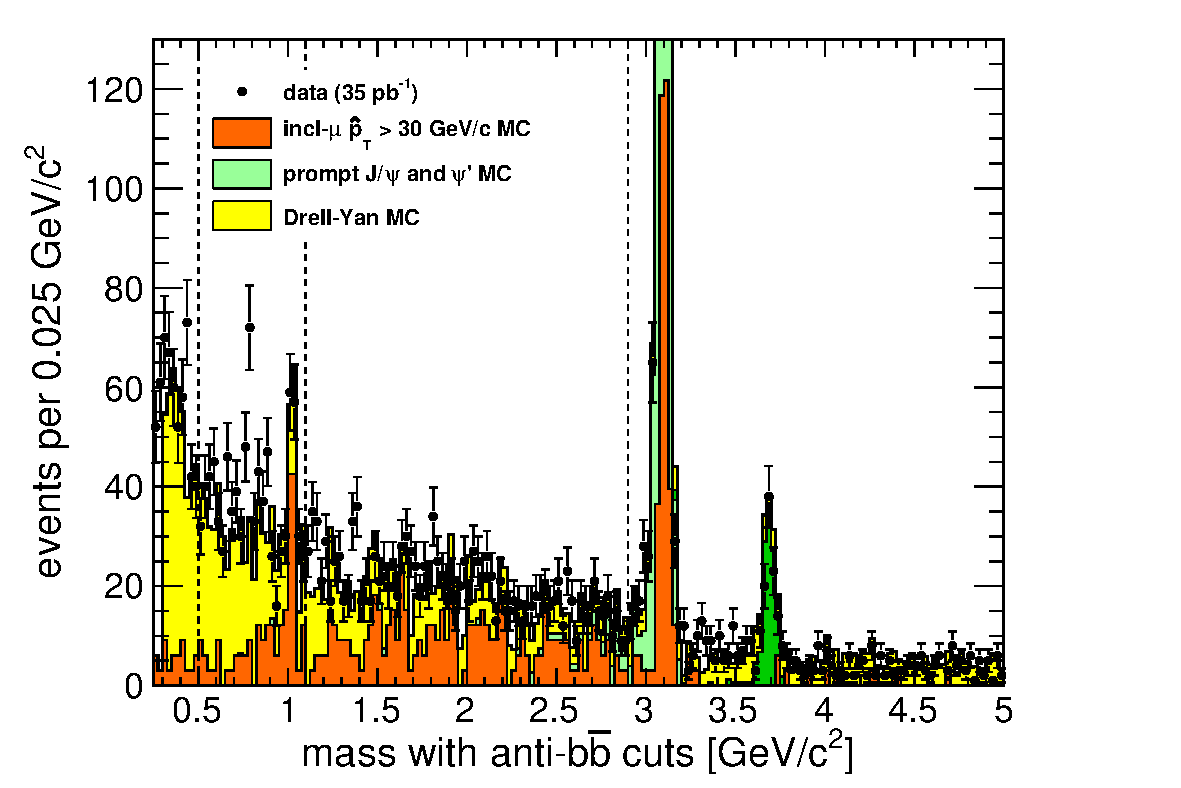
\includegraphics[width=0.33\linewidth]{support_mass_antibbbar.pdf}
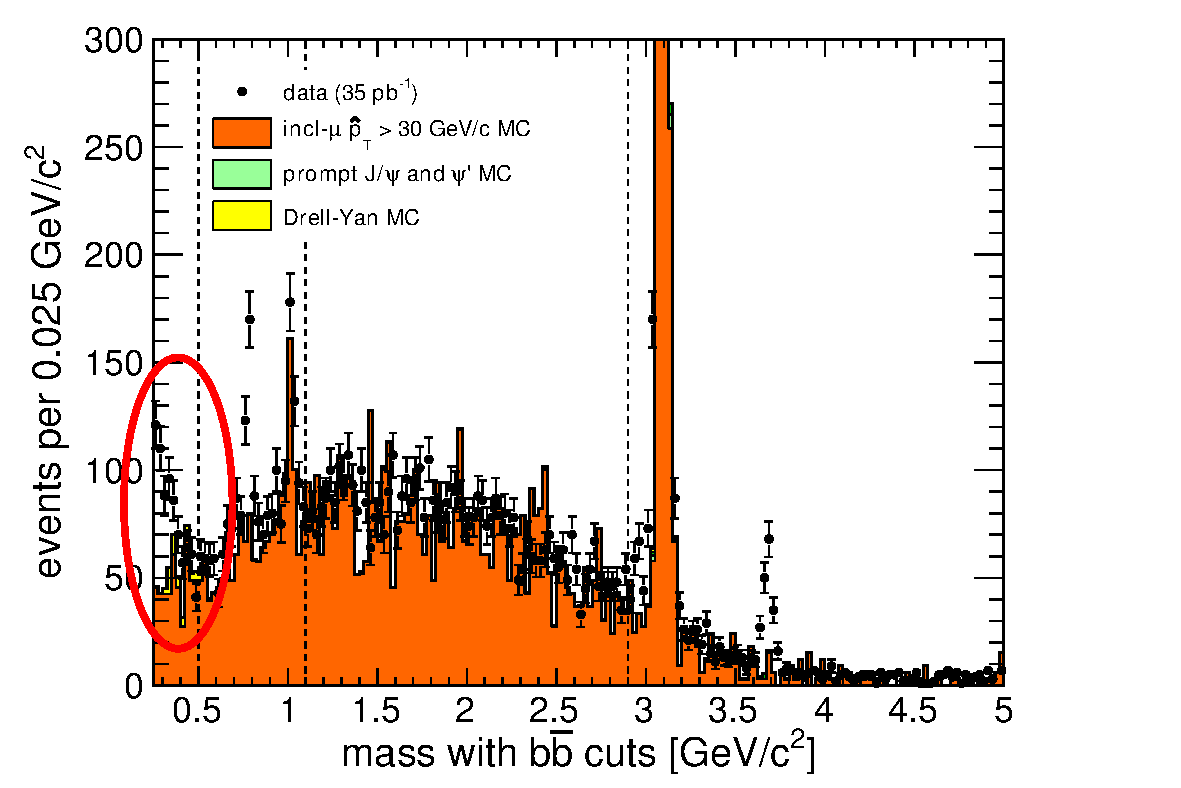
\includegraphics[width=0.33\linewidth]{support_mass_bbbar.pdf}

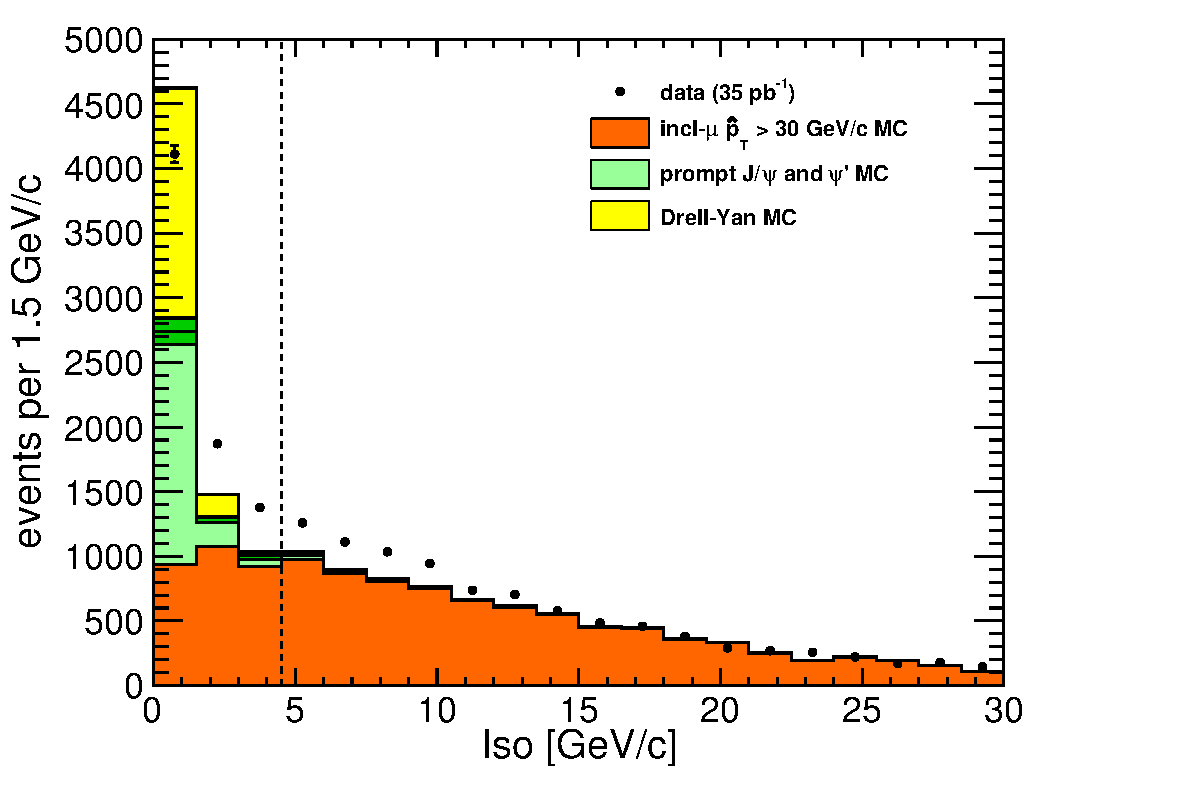
\includegraphics[width=0.33\linewidth]{support_iso_all.pdf}
\includegraphics[width=0.33\linewidth]{support_iso_continuum.pdf}
\includegraphics[width=0.33\linewidth]{support_iso_lowmass.pdf}

\includegraphics[width=0.33\linewidth]{support_lxy_all.pdf}
\includegraphics[width=0.33\linewidth]{support_lxy_continuum.pdf}
\includegraphics[width=0.33\linewidth]{support_lxy_lowmass.pdf}
\end{frame}

\begin{frame}
\frametitle{Low-mass dimuons}

\begin{itemize}
\item $b\bar{b}$ cuts do not bias the shape of the mass spectrum for real $b\bar{b}$ (left)
\item Drell-Yan/prompt resonances and $b\bar{b}$ components scale proportionally above $p_T > 40$~GeV/$c$ (right)
\end{itemize}

\includegraphics[width=0.5\linewidth]{support_bbbarcut_efficiency.pdf}
\includegraphics[width=0.5\linewidth]{support_bbbarcut_limits.pdf}
\end{frame}

\begin{frame}
\frametitle{Region (a-2): high $\mu$ multiplicity}

\begin{itemize}
\item When we add tracks to the mu-jet to simulate fake muons, do they have the same kinematics as muons?
\item Yes, they do (except for the highest-$p_T$ muon, which is special because it is selected to satisfy the trigger).
\end{itemize}

\begin{center}
\includegraphics[width=0.75\linewidth]{support_mujetplustracks_ptspectra.pdf}
\end{center}
\end{frame}

\begin{frame}
\frametitle{Region (a-2): high $\mu$ multiplicity}

\begin{itemize}
\item Another control region: the off-diagonal part of the mass-mass plane
\item Only one event outside of blinded region; it has low mass, as expected of fakes
\item Three of these muons have only 2 segments each (the minimum number)
\end{itemize}

\vfill
\includegraphics[height=4.5 cm]{data_quadmu_wholecontrol.pdf} \hfill
\includegraphics[height=4.5 cm]{quadmu_control_eventdisplay.png}
\end{frame}

\begin{frame}
\frametitle{Region (b-1): two dimuons}

\begin{itemize}
\item Demonstration that the distribution factorizes with
  high-statistics $b\bar{b} \to 2\mu \, 2\mu$ MC
\end{itemize}

\includegraphics[height=4 cm]{mc_dimudimu_wholecontrol.pdf} \hfill
\includegraphics[height=4 cm]{mc_wholecontrolregions_factorize.pdf}
\end{frame}

\end{document}
